\chapter[The Polar Front]{The Polar Front as a major biogeographic boundary in the Southern Ocean} 
\label{ch:polarfront}

\previouslypublished{Sections of this chapter have been previously published in \bibentry{Wilkins:2012wg}.}

\section{Abstract}

The \ac{PF} is a major oceanographic feature of the \ac{SO}, dividing surface water masses with distinct physicochemical characteristics.
To confirm and characterise the \ac{PF}'s role as a biogeographic barrier in the \ac{SO}, sixteen metagenomic samples were collected on a latitudinal transect from waters near Hobart, Australia (44\textdegree{} S) to near the Mertz Glacier, Antarctica (67\textdegree{} S).
The samples were shotgun sequenced, and the community composition and functional potential of the captured microorganisms were analysed.
The SAR11 and SAR116 clades and the cyanobacterial genera \genus{Prochlorococcus} and \genus{Synechococcus} were strongly overrepresented north of the \ac{PF}.
Conversely, the \ac{GSO-EOSA-1} complex, the phyla Bacteroidetes and Verrucomicrobia and order Rhodobacterales were overrepresented in waters south of the \ac{PF}. 
Functions enriched south of the \ac{PF} included a range of transporters, sulphur reduction and histidine degradation to glutamate, while branched-chain amino acid transport, nucleic acid biosynthesis and methionine salvage were overrepresented north of the \ac{PF}.
The taxonomic and functional characteristics suggested a shift of primary production from cyanobacteria in the north to eukaryotic phytoplankton in the south, and reflected the different trophic states of the two regions. 
Overall, this study supported the \ac{PF} as a defining biogeographic feature of the \ac{SO}.

%reset acronyms
\glsresetall

\section{Introduction}

The surface waters of the \ac{SO} consist of zones separated by circumpolar fronts, the locations of which vary with time and longitude \cite{Whitworth:1980wo,Orsi:1995va,Sokolov:2002tc}.
From north to south, the major fronts are the \ac{STF}, the \ac{SAF} and the \ac{PF} \figref{fig:oceanographymap}.
The \ac{SAF} and \ac{PF} are associated with the \ac{ACC}, the world's largest ocean current and a defining oceanographic feature of the \ac{SO}.
Anthropogenic climate change may be driving the warming and freshening of the \ac{ACC} \cite{Boning:2008il}.
It may also be shifting the \ac{ACC} and associated fronts poleward; the mean path of the current has moved \textapprox{}50 km south since the 1950s \cite{Gille:2002fr}.
If this migration continues, by 2100 it will have displaced a volume of water south of the \ac{ACC} approximately equivalent to the Arctic Ocean \cite{Fyfe:2005vp}.

Climate change may also be affecting the surface regions defined by these fronts.
The major surface zones of the \ac{SO} are the \ac{SAZ}, between the \ac{STF} and \ac{SAF}; the \ac{PFZ}, between the \ac{SAF} and the \ac{PF}; and the \ac{AZ}, between the \ac{PF} and the Antarctic continent \figref{fig:oceanographymap}.
These zones have different physicochemical properties, such as density, salinity, temperature and nutrient concentrations \cite{Sokolov:2002tc}, and the fronts represent stepwise transitions in these properties \cite{WhitworthIII:1987ky}.
However, as a consequence of climate change, waters on the poleward side of the \ac{ACC} have become warmer and more saline, while those to the north cooler and fresher \cite{Boning:2008il}.

The \ac{PF} has been suggested to be a major biogeographic boundary in the distribution and abundance of both zooplankton \cite{Chiba:2001un,Hunt:2001vp,Esper:2002ui,Ward:2003db} and bacterioplankton \cite{Selje:2004ka,Abell:2005ji,Giebel:2009hr,Weber:2010fi}.
The effects of climate change on the physical oceanography of the \ac{SO} may therefore have global ecological significance, particularly as the \ac{SO} is a major site for sequestration of anthropogenic \ce{CO_{2}} \cite{Sabine:2004fz,MikaloffFletcher:2006ct} through both physicochemical processes and the microbe-driven ``biological pump'' of \ce{CO_{2}} fixation \cite{Thomalla:2011hi}, potentially forming a feedback loop \cite{Cox:2000ko}.
However, the microbial assemblages that inhabit the \ac{SO} are generally poorly understood, and their diversity and functional capacity poorly characterised \citep[reviewed in][]{Murray:2007db}.
A community-level understanding is needed to predict the effects of a shifting \ac{ACC} on the distribution, abundance and ecosystem functions of microorganisms.

Large scale metagenome surveys have not previously been performed in the \ac{SO}.
Compared to traditional environmental microbiological methods such as culture-based or DGGE surveys, metagenomic studies are able to offer both deeper (capture of sequence from rare taxa) and broader (larger sample sizes with greater statistical significance) data on the taxonomic makeup and functional capacities of marine microbial communities \citep[e.g.][]{Rusch:2007ez,Angly:2006wf,Dinsdale:2008cd}.
Metagenome sampling is also better suited to large-scale biogeographic studies, as it allows large numbers of samples to be taken across broad spatial and temporal scales with uniform sampling, storage and processing, compared to e.g.\ culture-based methods where technical replicability is more difficult.

This project is part of a metagenomic survey of the \ac{SO} begun in the austral summer of 2006, based on the sampling design of the \ac{GOS} \cite{Rusch:2007ez}.
The \ac{GOS} sampling strategy involves size fractionation of plankton assemblages by passing seawater through a 20 \micron{} prefilter then capturing planktonic biomass on sequential 3.0 \micron{}, 0.8 \micron{} and 0.1 \micron{} filter membranes.
As well as allowing deeper sequencing of metagenomes and thus better representation of low-abundance taxa \cite{Rusch:2007ez}, this approach allows comparison to other samples collected using the \ac{GOS} methods \citep[e.g.][]{Brown:2012gna}.
This study will thus focus on the 0.1--20 \micron{} fraction of the sampled microbial assemblages.

\section{Methods}
\subsection{Sampling and metagenomic sequencing}

Sampling\footnote{Sampling was performed by Jeffrey M. Hoffman and Jeffrey B. McQuaid.} was conducted on board the RSV \emph{Aurora Australis} during \ac{AAD} cruise V3 \ac{CEAMARC} / \ac{CASO} from 13 December 2007--25 January 2008. 
This cruise occupied the SR3 latitudinal transect from waters near Hobart, Australia (\textapprox{}44\textdegree{} S) to the Mertz Glacier polynya, Antarctica (\textapprox{}67\textdegree{} S) within a longitudinal range of \textapprox{}140--150\textdegree{} E.
Sixteen samples were obtained within this range \figref{fig:samplemap}.

% the sample map
\begin{figure}[!ht]
  \centering
  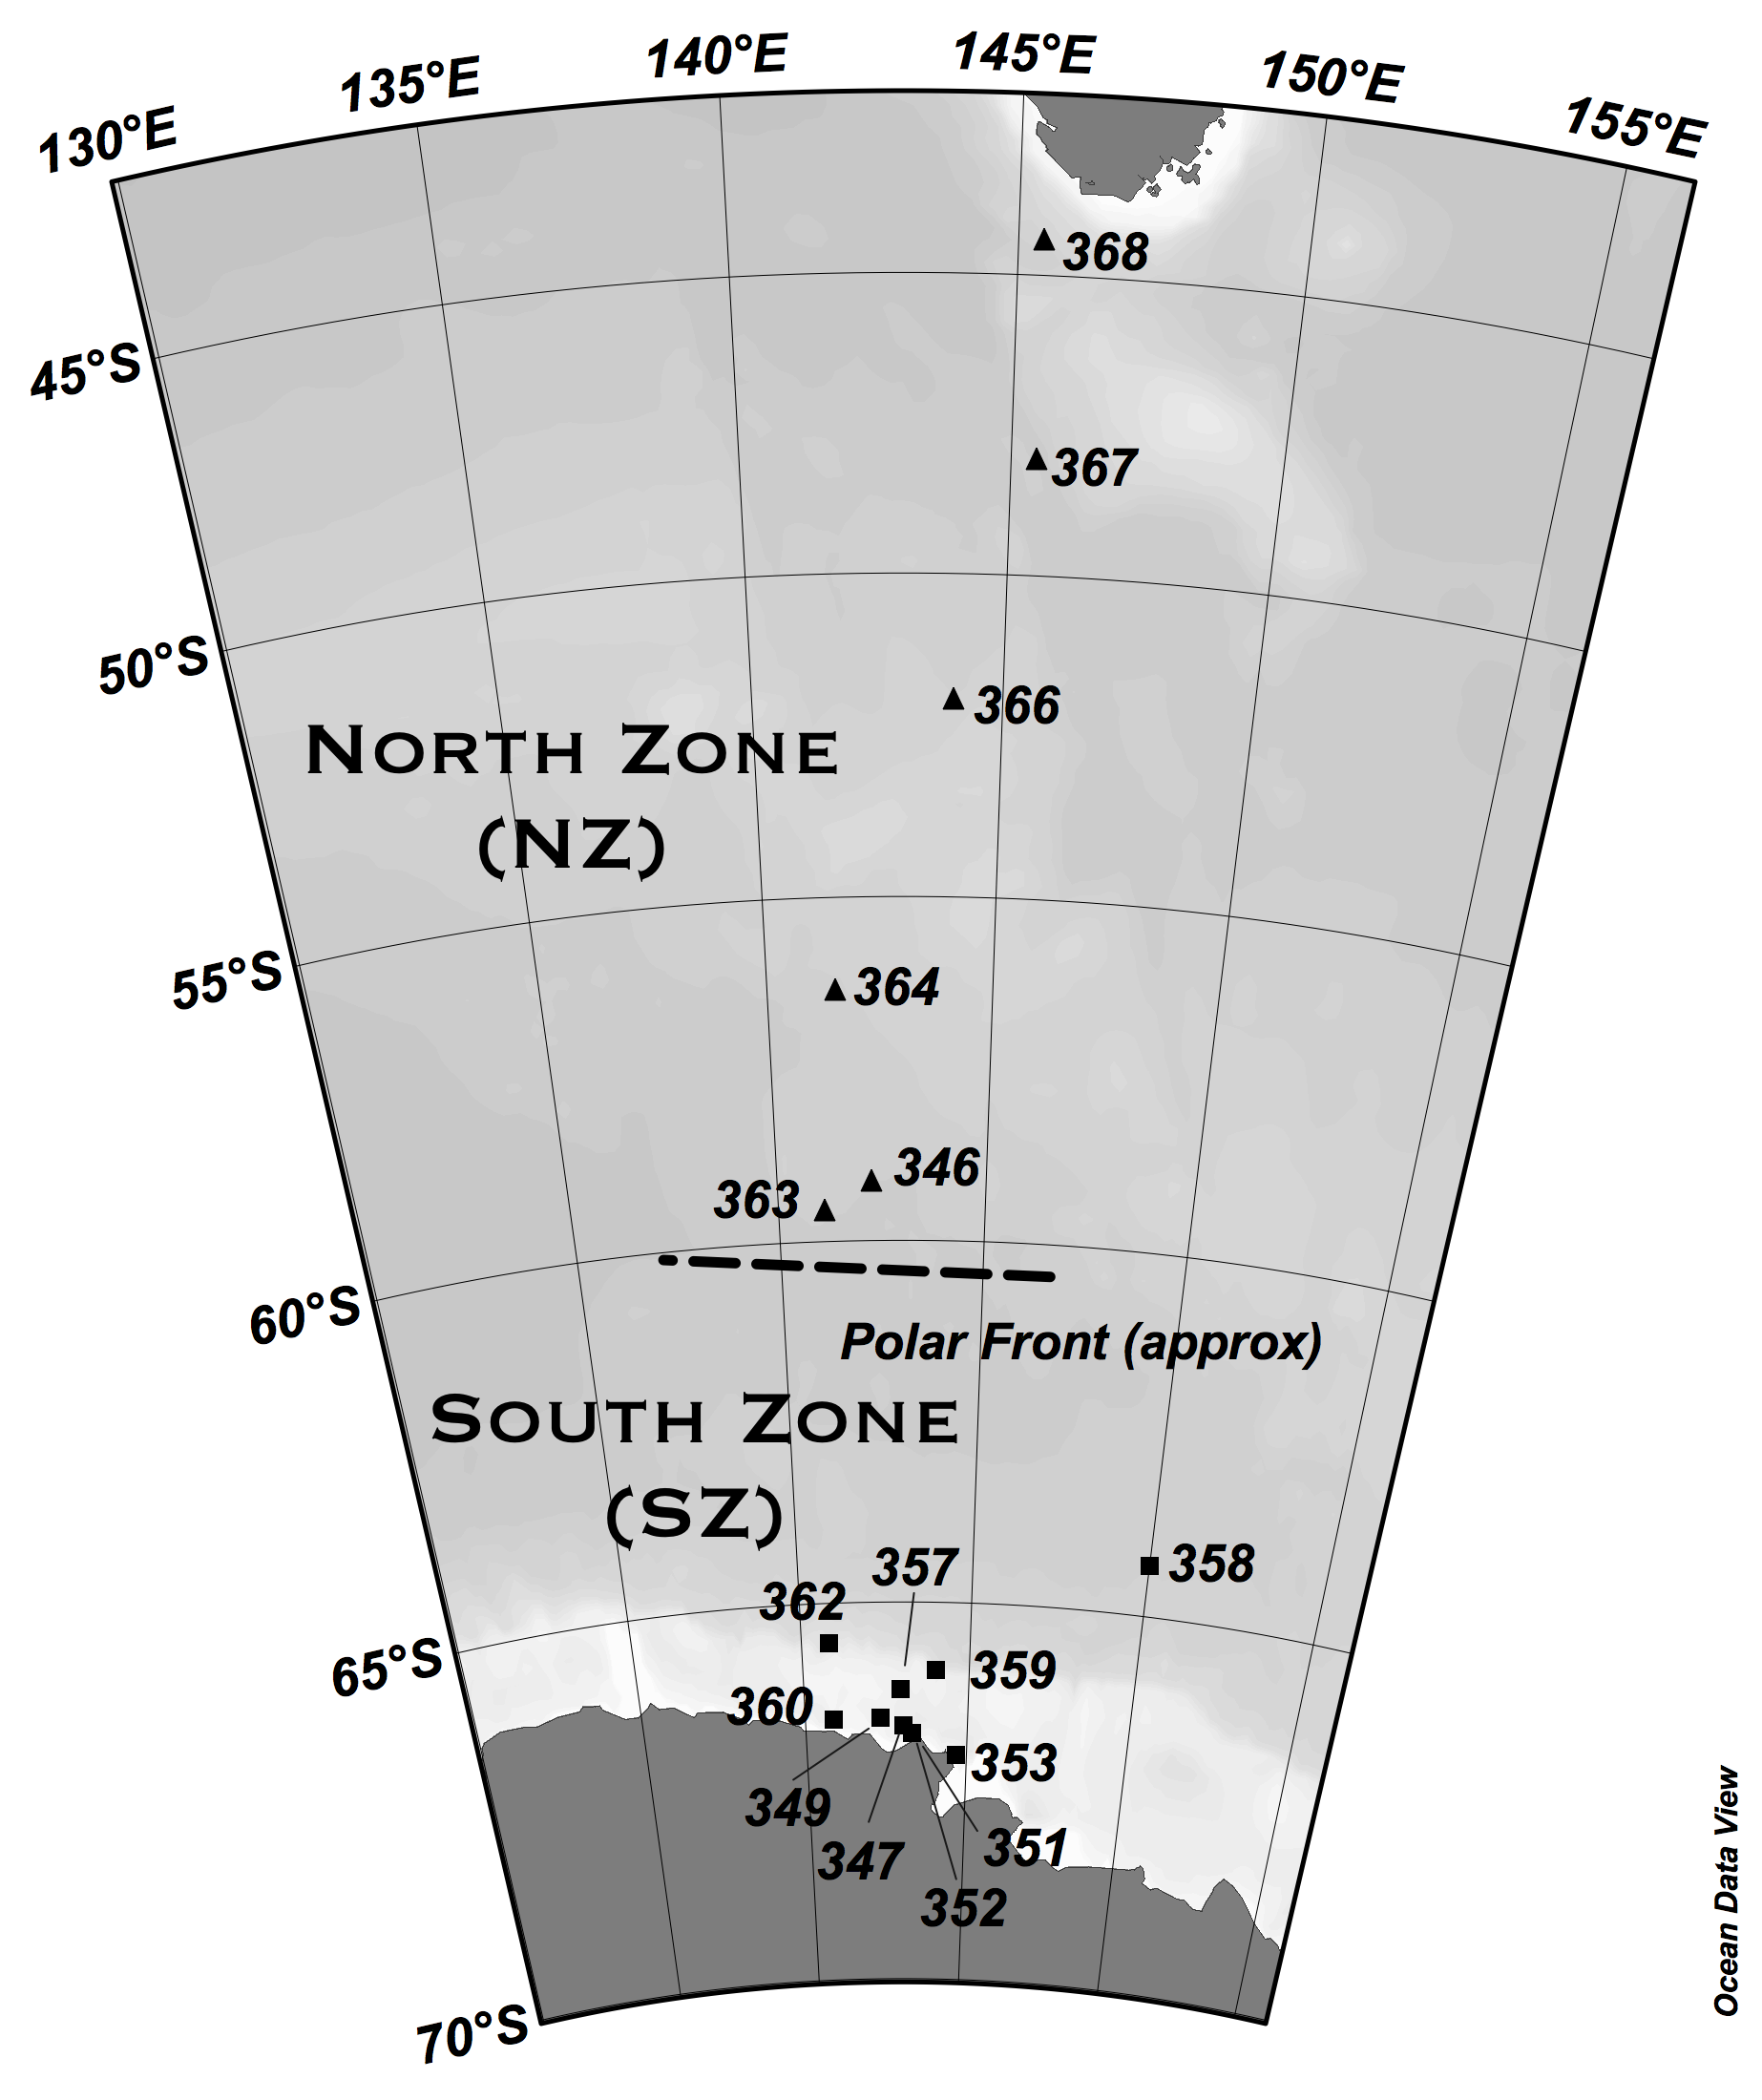
\includegraphics[width=\textwidth]{../polarfront/samplemap.png}
  \caption[Map showing sites of seawater samples used in the Polar Front study]{Sites of seawater samples used in this study. 
  Squares indicate surface samples from the North Zone; crosses samples from the South Zone. 
  The dashed line represents the Polar Front.}
  \label{fig:samplemap}
\end{figure}


A range of physicochemical data were recorded by integrated instruments on the RSV \emph{Aurora Australis} including water column depth, water temperature, salinity, fluorescence and meteorological conditions \tabref{tab:samplelist}.
These data were used to locate the \ac{PFZ} based on a surface temperature gradient of \textapprox{}1.35 \textdegree{}C across a distance of 45--65 km, placing the \ac{PF} at approximately 59.70\textdegree{} S, consistent with previous descriptions \cite{Moore:1999to,Sokolov:2002tc}.
Samples were accordingly grouped into ``North'' and ``South'' zones \tabref{tab:samplelist}.
The \ac{NZ} represents waters from the Subtropical, Subantarctic and \ac{PFZ} regions, while the \ac{SZ} represents the \ac{AZ}.

\begin{sidewaystable}
\sffamily
\caption[Details of samples used in Polar Front study]{\sffamily{}Sampling time, location and physicochemical properties of samples used in this study.
All data were retrieved from underway instruments aboard the RSV \textit{Aurora Australis}.}
\label{tab:samplelist}
\smallskip
\begin{tabularx}{\textheight}{lllXXXXXXXX}
\toprule
\textbf{Sample} & \textbf{Zone} & \textbf{Date} & \textbf{Latitude} & \textbf{Longitude} & \textbf{Water \linebreak Column \linebreak Depth (m)} & \textbf{Sample Depth (m)} & \textbf{Temperature (\textdegree{}C)} & \textbf{Salinity (PSU)} & \textbf{Fluorescence \linebreak (\textmu{}gL\textsuperscript{\textminus{}1})} & \textbf{Volume \linebreak filtered (L)}\\
\midrule

346 & North & 20/12/2007 & \textminus{}59.31 & 142.59 & 4294 & 2 & 2.9 & 33.75 & 0.3 & 500\\
347 & South & 23/12/2007 & \textminus{}66.02 & 142.74 & 450 & 2 & 0.6 & 34.20 & 4.0 & 250\\
349 & South & 27/12/2007 & \textminus{}66.57 & 142.32 & 370 & 1.5 & \textminus{}1.3 & 34.40 & 2.3 & 250\\
351 & South & 28/12/2007 & \textminus{}66.56 & 143.43 & 823 & 1.5 & \textminus{}0.6 & 34.30 & 1.3 & 500\\
352 & South & 29/12/2007 & \textminus{}66.77 & 143.32 & 164 & 2.5 & \textminus{}0.8 & 34.30 & 3.1 & 500\\
353 & South & 30/12/2007 & \textminus{}67.05 & 144.68 & 180 & 2 & \textminus{}1.8 & 34.40 & 0.3 & 500\\
357 & South & 05/01/2008 & \textminus{}66.17 & 143.02 & 580 & 2 & \textminus{}0.4 & 34.15 & 2.5 & 500\\
358 & South & 09/01/2008 & \textminus{}64.30 & 150.03 & 3550 & 2 & 0 & 33.55 & 0.5 & 500\\
359 & South & 12/01/2008 & \textminus{}66.19 & 143.53 & 540 & 2 & \textminus{}0.2 & 34.21 & 2.5 & 500\\
360 & South & 13/01/2008 & \textminus{}66.58 & 141.02 & 316 & 2 & \textminus{}0.7 & 34.04 & 6.2 & 500\\
362 & South & 19/01/2008 & \textminus{}65.54 & 140.83 & 1064 & 2 & 0.7 & 32.20 & 0.5 & 500\\
363 & North & 22/01/2008 & \textminus{}60.00 & 141.31 & 4473 & 2 & 3.3 & 33.77 & 0.1 & 500\\
364 & North & 23/01/2008 & \textminus{}56.70 & 141.88 & 3693 & 2 & 4 & 33.70 & 0.5 & 500\\
366 & North & 24/01/2008 & \textminus{}52.02 & 144.14 & 3180 & 2 & 7.6 & 33.84 & 0.3 & 500\\
367 & North & 25/01/2008 & \textminus{}48.25 & 145.90 & 3490 & 2 & 11 & 34.43 & 0.2 & 500\\
368 & North & 26/01/2008 & \textminus{}44.72 & 145.78 & 3201 & 2 & 14.8 & 34.96 & 1.3 & 560\\

\bottomrule
\end{tabularx}
\end{sidewaystable}


At each station, \textapprox{}250--560 L of seawater was pumped from \textapprox{}1.5--2.5 m below the sea surface into drums stored at ambient temperature on deck. 
Seawater samples were prefiltered through a 20 \micron{} plankton net, then biomass was captured on sequential 3.0 \micron{} 0.8 \micron{} and 0.1 \micron{} 293 mm polyethersulfone membrane filters (Pall, Port Washington, USA), and immediately stored at \textminus{}20 \textdegree{}C \cite{Rusch:2007ez,Ng:2010cd}.

DNA extraction\footnote{DNA extraction was performed by Cynthia Andrews-Pfannkoch and others at the J.\ Craig Venter Institute.} was performed at the J.\ Craig Venter Institute (Rockville, USA) using a modified phenol-chloroform method as described in \citet{Rusch:2007ez}.
Shotgun sequencing was performed on a GS20 FLX Titanium platform (Roche, Branford, USA) also at the J.\ Craig Venter Institute as described in \citet{Lauro:2010jna}.
Perfect duplicate reads were removed using sffToCa (Celera Corporation, Alameda, USA),  read ends were trimmed with \softwarename{Lucy} \cite{Chou:2001ck}, and the bottom 8\% and top 3\% of reads ordered by length were removed as described in \citet{Lauro:2010jna}\footnote{Read quality filtering was performed by Federico M.\ Lauro and Matthew Z.\ DeMaere.}.

\subsection{Phylogenetic analysis of metagenomic data}

\subsubsection{\softwarename{blast} comparison to RefSeq database}

A subset of the RefSeq microbial (bacterial and archaeal) genome database (release 41, retrieved 31 May 2010 from \url{ftp://ftp.ncbi.nih.gov/refseq/release/}) was prepared by excluding sequences with the words ``shotgun'', ``contig'', ``partial'', ``end'' or ``part'' in their headers.
This is necessary to ensure only full and complete genomes yielded matches, as the \ac{GAAS} software tool used for later processing uses this assumption to estimate environmental genome sizes \citep[following][]{Angly:2009ip}.

The metagenomic reads from each sample were compared against this database using \softwarename{tblastx}, with default parameters except for: E-value threshold $1.0\times{}10^{-3}$, cost to open gap 11, cost to extend gap 1, masking of query sequence by \softwarename{SEG} masking with lookup table only.
\acp{OTU} in this study are thus defined as the best species match in RefSeq by these parameters.
The outputs of all \softwarename{tblastx} searches against RefSeq were processed by \softwarename{minspec}, and hits not belonging to the minimal \ac{OTU} sets were removed.

\subsubsection{OTU abundances and variance between zones}

The relative \ac{OTU} abundances for each sample were determined using the \softwarename{perl} script \ac{GAAS} \cite{Angly:2009ip}.
\ac{GAAS} estimates the relative abundance of \acp{OTU} from the number and quality of \softwarename{blast} matches (``hits'') to each \ac{OTU}, taking into account differences in genome size. 
This approach takes advantage of all sequencing reads in a shotgun metagenome, in contrast with marker-gene bases approaches (e.g.\ 16S), and allows relative abundances to be estimated on a ``one genome per cell'' basis, increasing the accuracy of these estimates.
\ac{GAAS} was run with the default settings. 
To normalise for reads which did not yield acceptable hits, the relative abundances for each sample were scaled by that sample's effective \softwarename{blast} hit rate.

A difficulty with the size fractionation approach is that relative abundances cannot be summed across fractions.
This is because each fraction almost certainly represents a different absolute number of cells.
If the relative abundances are summed, the apparent abundance of some \acp{OTU} could be distorted (visually demonstrated in \figreft{fig:fractionabundances}).
Thus, an \ac{OTU} profile was generated for each sample by encoding the scaled relative abundance of each \ac{OTU} from each size fraction as a separate variable.
This allows samples to be compared on the basis of community composition without introducing systematic biases.

\begin{figure}
\centering
\subfloat[\sffamily\label{fig:fractionabundancescellcount}]{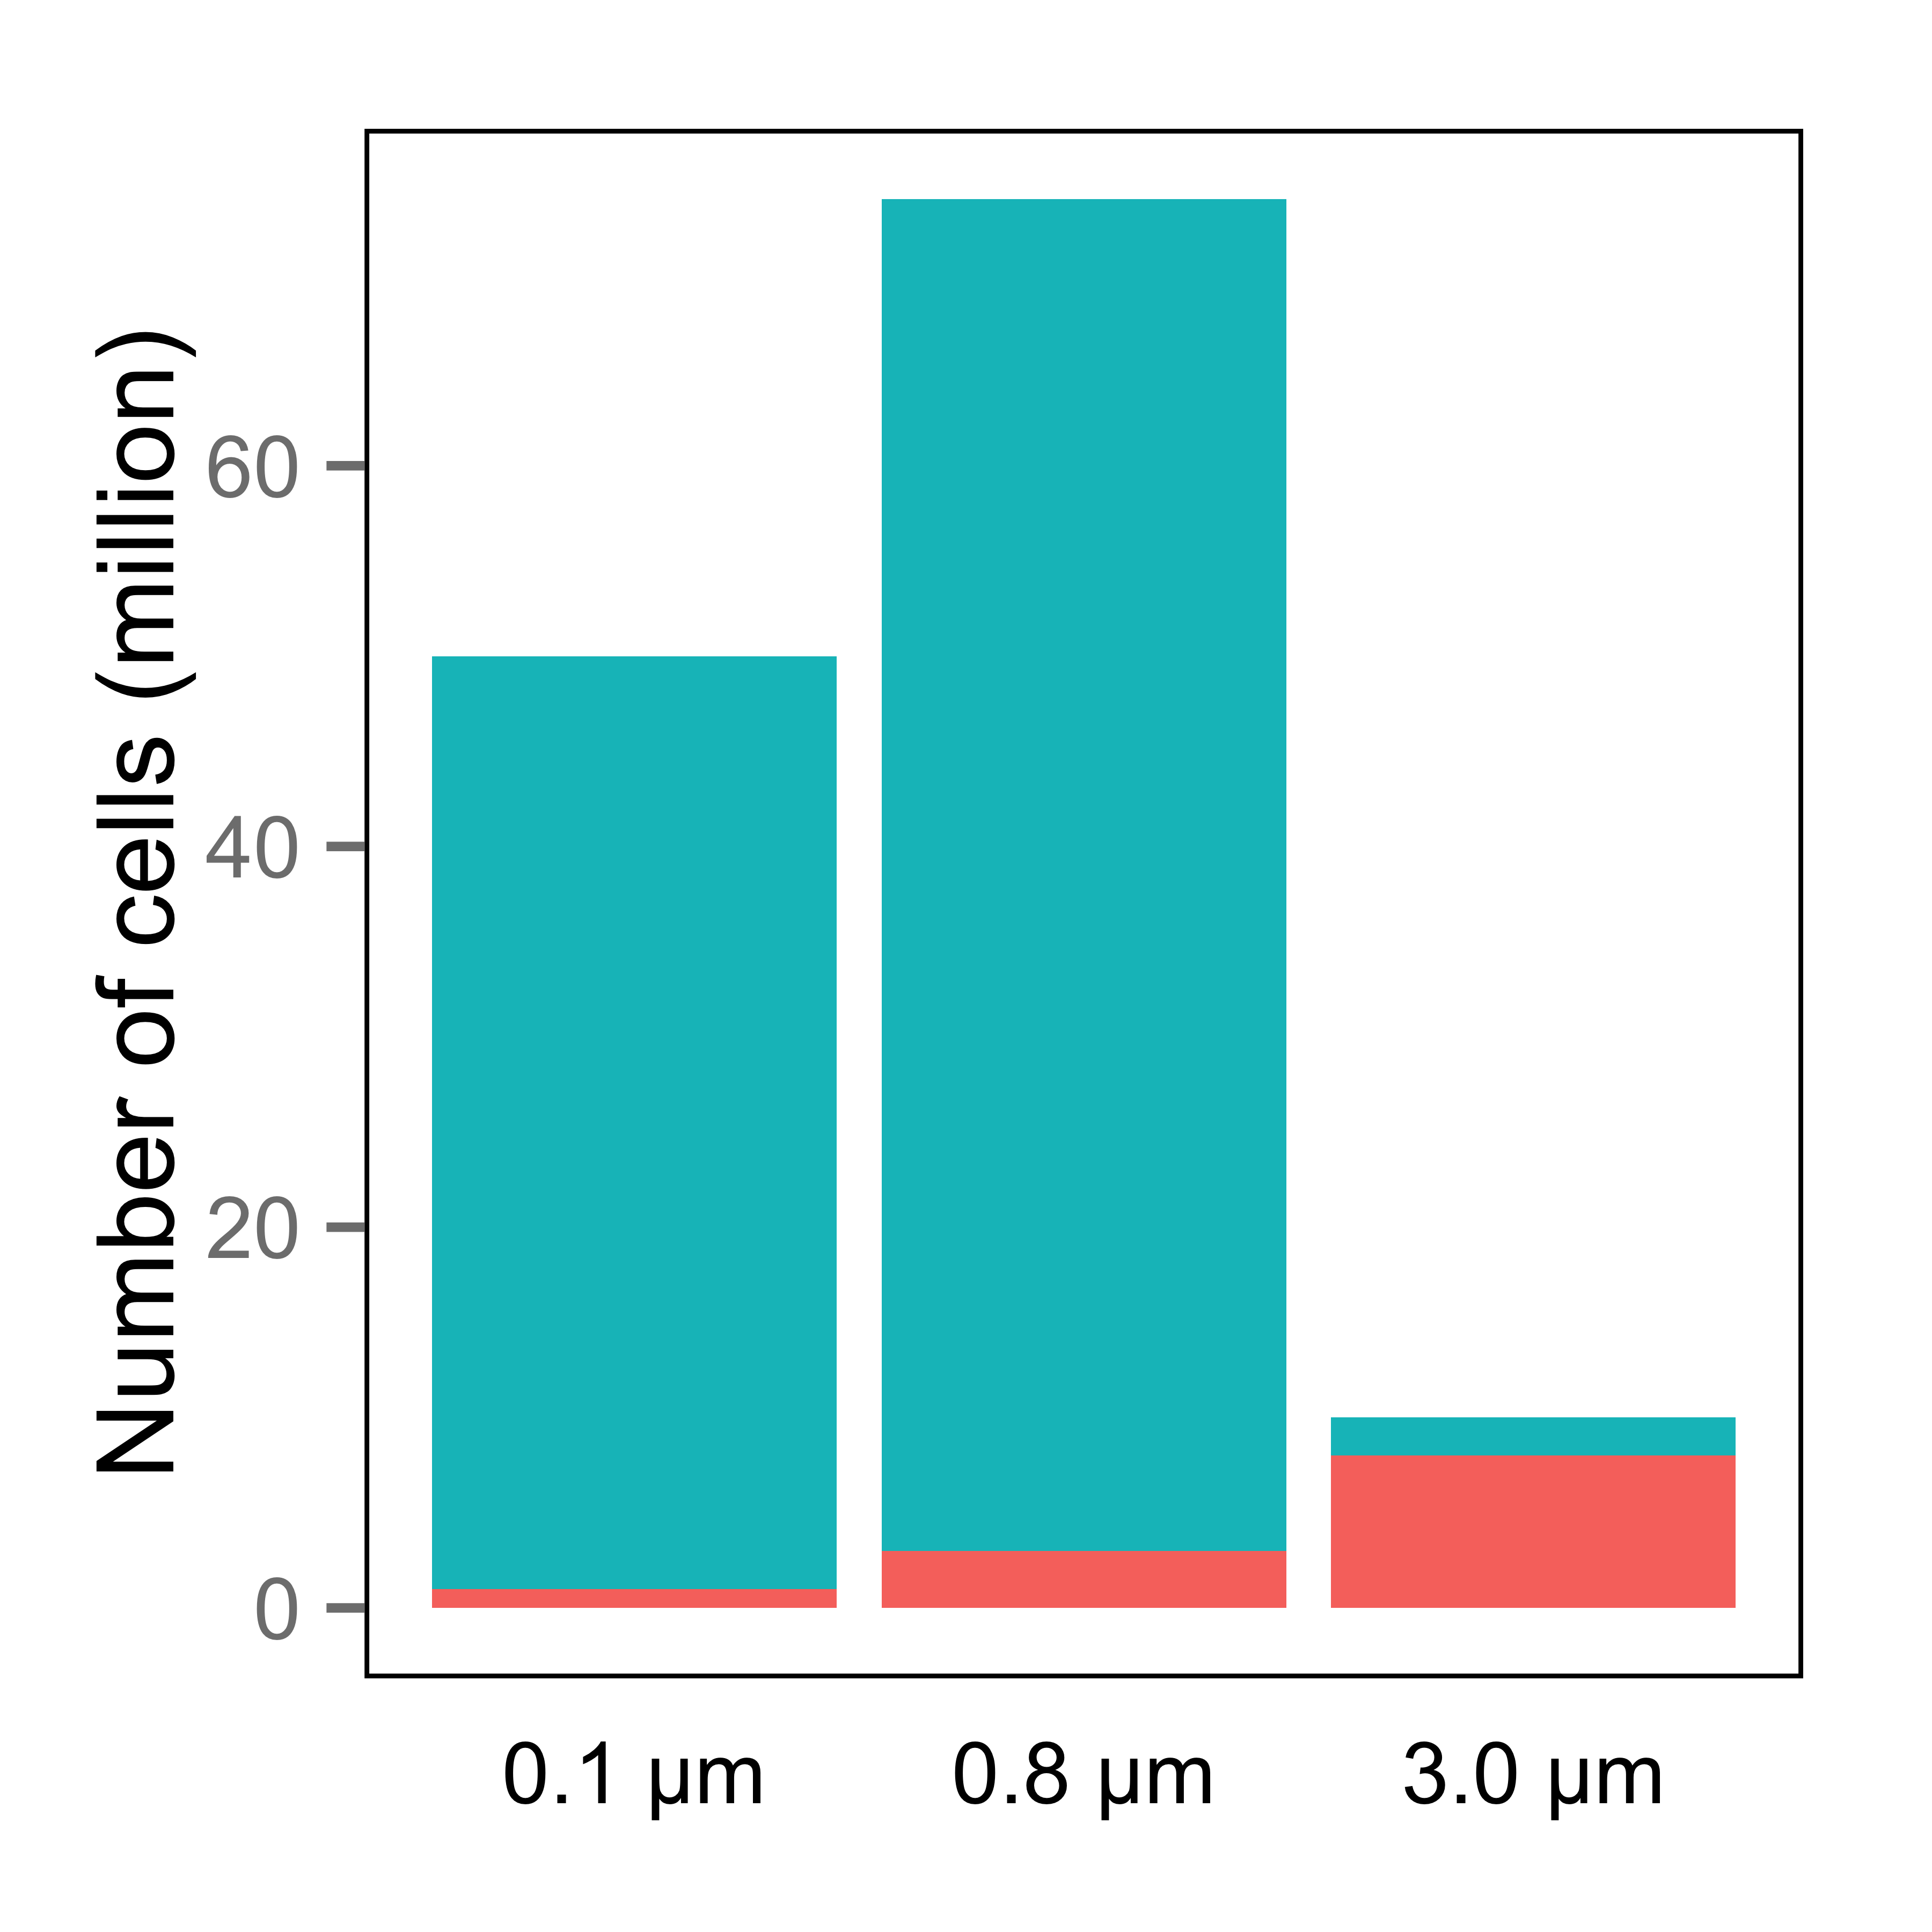
\includegraphics[scale=0.04]{../polarfront/fractionabundances1.png}}
\quad
\subfloat[\sffamily\label{fig:fractionabundancesrelative}]{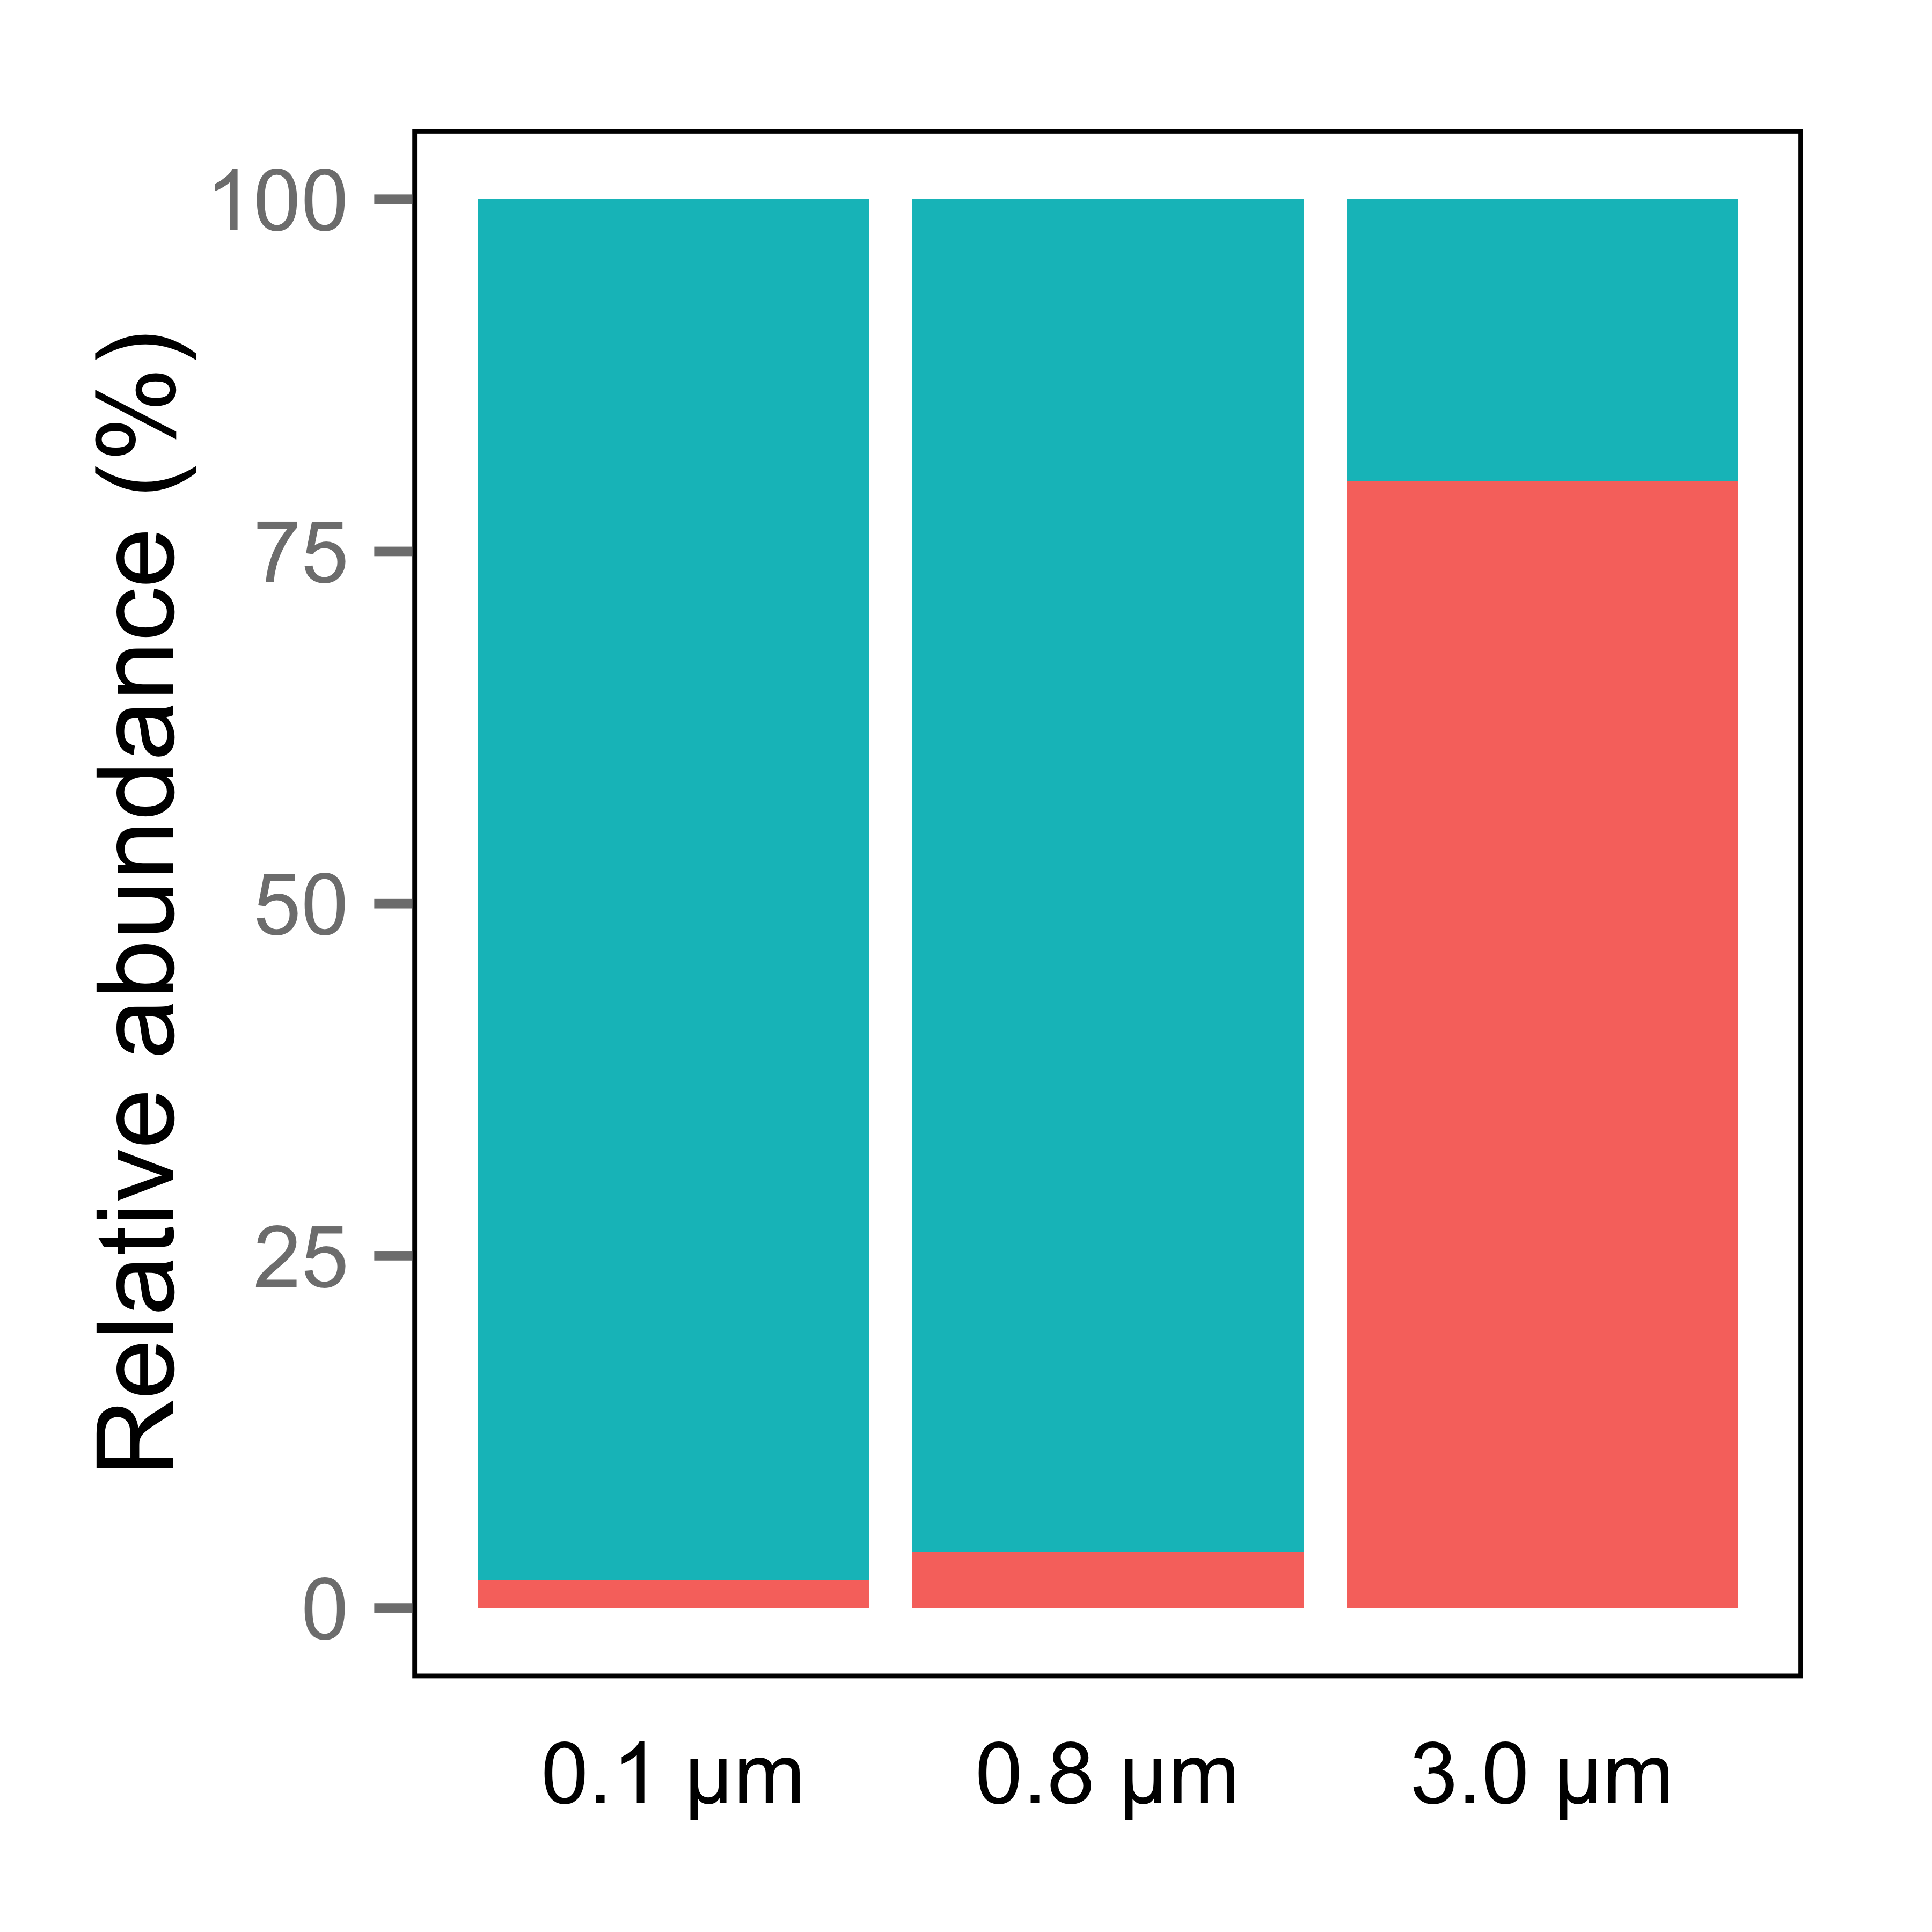
\includegraphics[scale=0.04]{../polarfront/fractionabundances2.png}}
\quad
\subfloat[\sffamily\label{fig:fractionabundancescombined}]{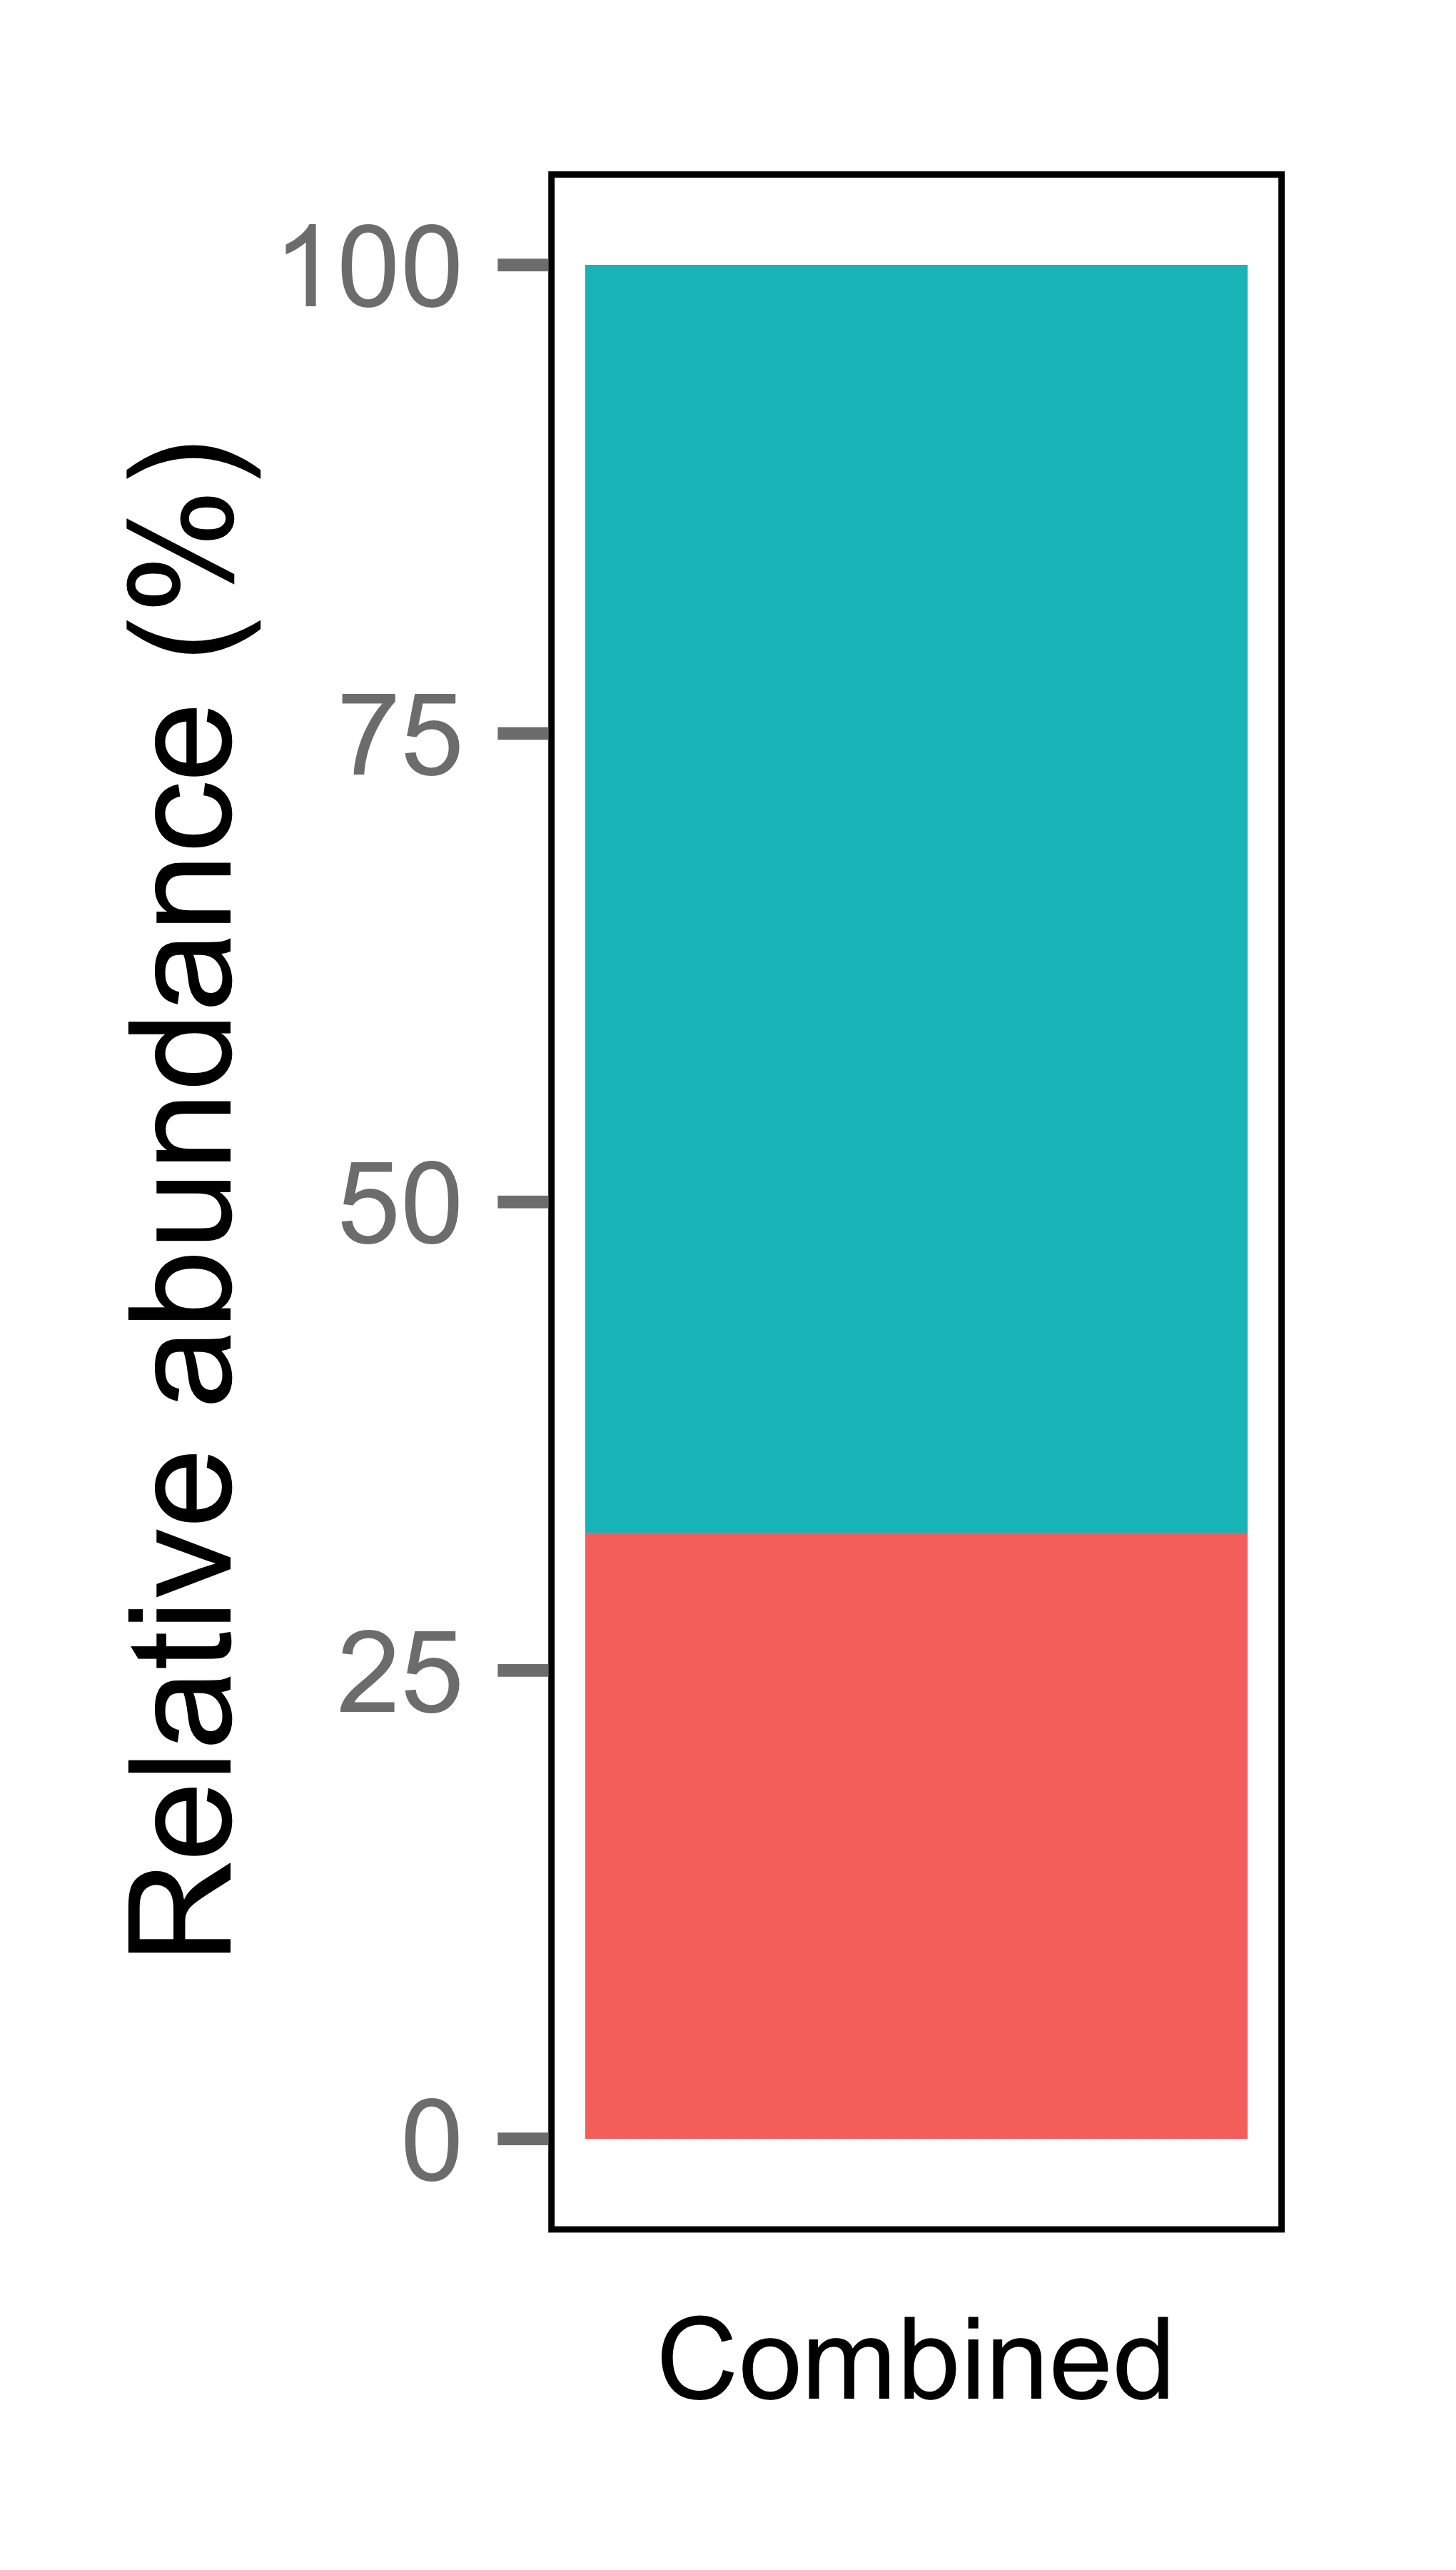
\includegraphics[scale=0.04]{../polarfront/fractionabundances3.png}}
\caption[Summing relative abundances across size fractions]{An example of distortion introduced by summing OTU relative abundances across size fractions. The red OTU composes only 15\% of the \emph{absolute} number of cells captured (a). However, it has a high \emph{relative} abundance (80\%) in the 3.0 \micron{} fraction (b). A metagenomic analysis without cell counts for each size fraction is only able to determine these relative abundances. If the relative abundances for each fraction are simply summed, the red OTU appears to compose 32\% of the community, more than twice the correct value (c). Without cell counts for each fraction, relative abundances cannot be summed between the fractions.}
\label{fig:fractionabundances}
\end{figure}


To test the hypothesis that the oceanic zones harbour significantly different communities, \ac{ANOSIM} with 999 permutations was performed on a standardised, log-transformed Bray-Curtis resemblance matrix of \ac{OTU} profiles.
\ac{SIMPER} analysis was performed to identify the contribution of individual \acp{OTU} to differences between the zones. 
All statistical procedures were performed in \softwarename{PRIMER 6} as described by \citet{Clarke:2001ut}.

\subsubsection{Fragment recruitment to verify \ac{OTU} identification}
Fragment recruitment to reference genomes was visualised as a precaution against unintended sequencing bias and to ensure the \ac{OTU} annotation pipeline was functioning as intended.
Plots of read recruitment depth on reference genomes were generated using a custom script in \softwarename{r} and \softwarename{perl}\footnote{This script, along with other accessory scripts used in this project, is open source and available at \url{https://github.com/wilkox/blast-tools}.}.
Samples from both the \ac{SZ} and \ac{NZ} were randomly selected and their 0.1 \micron{} fractions used as sources of recruited reads.
Three high-abundance and three low-abundance \acp{OTU} were randomly selected as the reference genomes.
As shotgun sequencing of a metagenome should be essentially random, it was predicted that these plots would show fairly even coverage of the reference genomes.
Genomes where all recruited reads were concentrated in a few small regions would be likely candidates for \acp{OTU} which were not present, but shared a small genomic region with an \ac{OTU} which was present, or possibly indicative of non-random priming during shotgun sequencing.

\subsubsection{Additional samples to test ``polynya hypothesis''}
Because many samples from the \ac{SZ} were taken in the region of the Mertz Glacier polynya, an alternative hypothesis for any difference observed between the \ac{SZ} and \ac{NZ} would be that the difference represented the effect of the polynya, rather than the \ac{PF}.
To test this, metagenomes from an additional set of samples collected\footnote{Collection was performed by Ricardo Cavicchioli, Federico M.\ Lauro and Mark V.\ Brown.} in a different project were obtained.
These samples were obtained in waters south of the \ac{PF} on different voyages and in a different longitudinal range \figref{fig:additionalsamples}, where the influence of the Mertz Glacier polynya could not account for any observed difference between the zones.
Sampling, DNA extraction and sequencing were\footnote{TODO who did this?} performed as described above, although only metagenomes from the 0.1--0.8 \micron{} size fraction were available.
The resulting metagenomic reads were compared to RefSeq and weighted relative abundances calculated with \ac{GAAS} as described above.

\begin{table}
\centering
\caption[Additional samples used to test polynya hypothesis]{Dates and locations of additional samples used to falsify the hypothesis that the Mertz Glacier polynya was responsible for the observed biogeographic partitioning.}
\label{tab:additionalsamples}
\begin{tabular}{lllll}
\toprule
\textbf{Sample} & \textbf{Date} & \textbf{\ac{AAD} Voyage Number} & \textbf{Latitude} & \textbf{Longitude}\\
\midrule
388 & 20/10/2008 & V1 2008--09 & $-63.8090$ & 115.1613\\
398 & 22/10/2008 & V1 2008--09 & $-64.8018$ & 112.3730\\
390 & 30/10/2008 & V1 2008--09 & $-64.8152$ & 80.7204\\
392 & 13/12/2008 & V2 2008--09 & $-64.1826$ & 76.4537\\
393 & 15/12/2008 & V2 2008--09 & $-55.2573$ & 74.2531\\
\bottomrule
\end{tabular}
\end{table}


Two \ac{ANOSIM} tests were performed on the standardised and log-transformed Bray-Curtis resemblance matrices of the samples' \ac{OTU} abundance profiles and similarly prepared matrices representing only the 0.1 \micron{} fractions of the \ac{SZ} and \ac{NZ} samples.
In the first \ac{ANOSIM} test (``polynya hypothesis''), all samples from the Mertz Glacier polynya region (i.e.\ all \ac{SZ} samples except 358) were grouped together, while the samples from the open ocean were placed in a separate group.
In the second test (``\ac{PF} hypothesis''), the samples were grouped by their location relative to the \ac{PF}.

\subsection{Functional analysis of metagenomic data}

\subsubsection{\softwarename{blast} comparison to KEGG database}

In order to identify functional differences between the zones, the set of metagenomic reads from each sample was compared against the \ac{KEGG} GENES database (retrieved 2 July 2010 from \url{ftp://ftp.genome.jp/pub/kegg/genes/fasta/genes.pep}) with \softwarename{blastx}, with default parameters except for: maximum number of database sequence alignments 10; E-value threshold $1.0\times10^{-3}$; gap opening penalty 11; gap extension penalty 1; masking of query sequence by \softwarename{SEG} masking for lookup table only.

\subsubsection{Analysis of functional potential}

Genes identified by \softwarename{blastx} were aggregated to \ac{KEGG} ortholog groups according to the \ac{KEGG} Orthology schema (\url{ftp://ftp.genome.jp/pub/kegg/genes/ko}, retrieved Mar 29 2011), and ortholog group abundances calculated for each sample. 
Following \citet{Coleman:2010jj}, a read was considered a hit to a given ortholog group if the top three hits for that read (or all hits if fewer than three total hits) were to genes from the same ortholog group, and had bit scores \textgreater{} 40. 
If the bit score difference between any two top hits was greater than 30, only the hits above this difference were considered.

Ortholog group counts were then used to calculate the abundance of KEGG modules.
Because many ortholog groups are members of more than one module, the abundance $a_m$ of each module $m$ was calculated as 
\[
a_{m}=\sum_{K=1}^{n}\frac{C_{K}}{M_K}
\]
where $n$ is the number of ortholog groups $K$ belonging to module $m$, $C_{K}$ is the number of hits to ortholog group $K$, and $M_{K}$ is the total number of modules to which $K$ belongs.
To account for differences in sequencing depth between samples, module abundances were scaled to 500,000 reads per sample.
To test the hypothesis that the \ac{NZ} and \ac{SZ} harbour significantly different functional potential, one-way \ac{ANOSIM} with 999 permutations was performed as above on a standardised, log-transformed Bray-Curtis distance resemblance matrices of the module and ortholog group profiles.
\ac{SIMPER} was performed as above to identify modules which contributed highly to the variation in functional potential between the two zones.

\subsubsection{Taxonomic decomposition}

To link modules with a high contribution to variance or otherwise of interest to specific \acp{OTU} (``taxonomic decomposition''), a script was written in \softwarename{perl} to decompose each module to its constituent ortholog groups, then each ortholog group to each representative gene sequence in the \ac{KEGG} GENES database.
Because each \ac{KEGG} GENES sequence is associated with a particular organism, this allowed the abundance of each module to be decomposed into the relative contribution from each of these organisms.
Functional contributions could then be putatively assigned to \acp{OTU}, including those which were not identified in the taxonomic analysis, as the database included gene sequences for organisms for which a full genome was not available.
To aid interpretation of these results, the taxonomic decompositions for some modules were aggregated to higher taxonomic ranks, such as class or family.

\section{Results}

\subsection{Metagenomic sequencing}
6.6 Gbp of sequence data representing microorganisms in the size range 0.1--3.0 \micron{} was obtained from 16 samples. 
After removing low-quality reads, 157,507--597,689 reads remained per sample (mean 354,399) with lengths ranging from 100 to 606 bp (mean 378 bp).

\subsection{Phylogenetic analysis of metagenomic data}

The proportion of reads in each sample that yielded hits to RefSeq ranged from 25--85\% (mean 62\%).
The most abundant \acp{OTU} in each sample are given in \tabreft{tab:topotus} and a full list of \ac{OTU} abundances in the supplementary material \suppfile{PF-all-OTUs.txt}.
All samples and size fractions exhibited very low \ac{OTU} evenness \figref{fig:rankabundance}.

\begin{sidewaystable}
\sffamily
\caption[Twenty most abundant \acp{OTU}]{\sffamily{}Relative abundances (as percentages) of the twenty most abundant \acp{OTU} identified in this study, in each zone and size fraction.}
\label{tab:topotus}
\smallskip
\begin{tabularx}{\textheight}{Xlllllllll}
\toprule
OTU & \multicolumn{3}{c}{North} & \multicolumn{3}{c}{South} & \multicolumn{3}{c}{Deep}\\
\cmidrule(r){2-4}
\cmidrule(r){5-7}
\cmidrule(r){8-10}
& 0.1 \micron & 0.8 \micron & 3.0 \micron & 0.1 \micron & 0.8 \micron & 3.0 \micron & 0.1 \micron & 0.8 \micron & 3.0 \micron\\
\midrule

\candidatusfull{Pelagibacter ubique} HTCC1062 & 61.76 & 25.00 & 23.87 & 58.85 & 22.40 & 17.61 & 37.05 & 24.56 & 17.66\\
\speciesfull{Nitrosopumilus maritimus} SCM1 & 0.01996 & 0.01438 & 0.009508 & 1.076 & 1.309 & 1.210 & 19.09 & 9.463 & 17.77\\
\candidatusfull{Ruthia magnifica} str. Cm (\speciesfull{Calyptogena magnifica}) & 0.6699 & 0.6458 & 0.5484 & 2.987 & 2.616 & 1.025 & 3.945 & 4.601 & 2.264\\
\genus{Roseobacter} sp. OCh114 & 0.3125 & 2.932 & 1.588 & 0.4477 & 3.994 & 2.657 & 0.1259 & 1.228 & 0.6792\\
\genus{Synechococcus} sp. CC9902 & 0.1081 & 9.837 & 4.973 & 0.0007484 & 0.004156 & 0.09733 & 0.002846 & 0.01502 & 0.01058\\
\speciesfull{Silicibacter pomeroyi} DSS-3 & 0.2578 & 2.286 & 1.154 & 0.3070 & 2.505 & 1.576 & 0.1224 & 0.9417 & 0.4988\\
\speciesfull{Gramella forsetii} strain KT0803 & 0.2412 & 1.210 & 1.755 & 0.4993 & 2.347 & 1.890 & 0.2078 & 0.6179 & 0.5173\\
\candidatusfull{Vesicomyosocius okutanii} strain HA & 0.4634 & 0.4642 & 0.2078 & 1.970 & 1.807 & 0.2174 & 2.480 & 2.662 & 1.167\\
\speciesfull{Robiginitalea biformata} strain HTCC2501 & 0.2751 & 1.099 & 1.297 & 0.4722 & 1.878 & 1.405 & 0.2265 & 0.6188 & 0.6946\\
\speciesfull{Flavobacterium psychrophilum} strain JIP02/86 & 0.1718 & 0.8409 & 1.224 & 0.4316 & 1.960 & 1.598 & 0.1599 & 0.4744 & 0.6001\\
\genus{Synechococcus} sp. CC9311 & 0.03014 & 4.624 & 4.409 & 0.0007221 & 0.002778 & 0.02764 & 0.001580 & 0.002863 & 0.009241\\
\candidatusfull{Puniceispirillum marinum} IMCC1322 & 0.6444 & 2.077 & 1.267 & 0.3586 & 1.377 & 0.7109 & 0.3425 & 1.062 & 0.5345\\
\genus{Silicibacter} sp. TM1040 & 0.2274 & 1.652 & 0.8738 & 0.2709 & 1.803 & 1.233 & 0.07665 & 0.5890 & 0.2957\\
\genus{Jannaschia} sp. DFL-12 & 0.1776 & 1.378 & 0.7350 & 0.2443 & 1.692 & 0.8009 & 0.07338 & 0.6515 & 0.3078\\
\speciesfull{Zunongwangia profunda} strain SM-A87 & 0.1522 & 0.7487 & 1.059 & 0.2968 & 1.410 & 1.204 & 0.1353 & 0.3478 & 0.4971\\
\genus{Colwellia} sp. 34H & 0.02345 & 0.3636 & 2.736 & 0.05207 & 0.5140 & 1.041 & 0.05137 & 0.4687 & 0.8013\\
\speciesfull{Coraliomargarita akajimensis} strain DSM 45221 & 0.03698 & 0.07573 & 0.1197 & 0.1154 & 1.543 & 1.680 & 0.02614 & 0.3040 & 0.2740\\
\genus{Jannaschia} sp. CCS1 & 0.1173 & 0.9344 & 0.4784 & 0.1711 & 1.230 & 0.8239 & 0.05865 & 0.4462 & 0.2118\\
\speciesfull{Pseudoalteromonas atlantica} strain T6c & 0.01251 & 0.4772 & 1.993 & 0.02270 & 0.4089 & 1.132 & 0.02634 & 0.2143 & 0.7459\\
\speciesfull{Saccharophagus degradans} strain 2-40 & 0.06532 & 0.4325 & 0.5429 & 0.1289 & 1.072 & 0.8663 & 0.07798 & 0.2844 & 0.3165\\
\speciesfull{Flavobacterium johnsoniae} strain UW101 & 0.08822 & 0.4220 & 0.6141 & 0.2034 & 0.9389 & 0.8578 & 0.07545 & 0.2255 & 0.3300\\
\speciesfull{Capnocytophaga ochracea} strain DSM 7271 & 0.1143 & 0.4830 & 0.5399 & 0.2314 & 0.8815 & 0.6814 & 0.08964 & 0.2840 & 0.5043\\
\genus{Marinomonas} sp. MWYL1 & 0.03777 & 0.2529 & 0.3026 & 0.1514 & 1.300 & 0.7006 & 0.07393 & 0.2439 & 0.2155\\
\speciesfull{Cellvibrio japonicus} strain Ueda107 & 0.05884 & 0.3080 & 0.3231 & 0.1155 & 0.9917 & 0.4713 & 0.06774 & 0.2981 & 0.2549\\
\speciesfull{Marinobacter hydrocarbonoclasticus} VT8 & 0.04093 & 0.2889 & 0.3883 & 0.08418 & 0.7195 & 0.3848 & 0.1250 & 0.6667 & 1.066\\
\speciesfull{Pseudoalteromonas haloplanktis} strain TAC125 & 0.01389 & 0.2505 & 0.8896 & 0.03427 & 0.3561 & 0.6530 & 0.1092 & 1.203 & 0.1503\\
\speciesfull{Teredinibacter turnerae} strain T7901 & 0.05665 & 0.3051 & 0.3081 & 0.1138 & 0.9174 & 0.5127 & 0.06558 & 0.2649 & 0.1885\\
\speciesfull{Acinetobacter baumannii} strain SDF & 0.004886 & 0.007187 & 0.4073 & 0.006260 & 0.04218 & 1.459 & 0.004285 & 0.01229 & 0.3155\\

\bottomrule
\end{tabularx}
\end{sidewaystable}

% the sample map
\begin{figure}
  \centering
  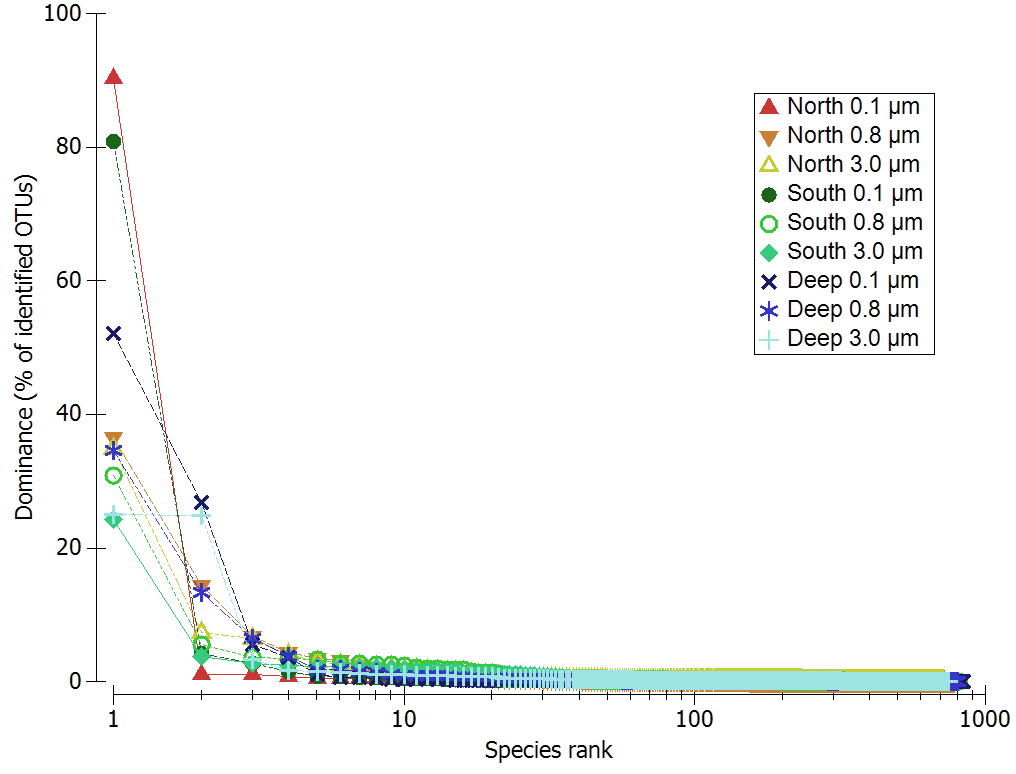
\includegraphics[width=\textwidth]{../polarfront/rankabundance.png}
  \caption[Rank-abundance curves for OTUs in each zone and size fraction]{Rank-abundance curves for OTUs identified in each zone and size fraction. The dominance of a given OTU is its relative abundance as a percentage of all identified OTUs. The x-axis is scaled logarithmically. Generated using \softwarename{PRIMER 6}.}
  \label{fig:rankabundance}
\end{figure}


\ac{ANOSIM} analysis showed that the zones harbor significantly different microbial communities (R = 0.45, p = 0.004). 
\ac{SIMPER} was performed in order to identify the contribution of individual \acp{OTU} to the difference between the \ac{NZ} and \ac{SZ}. 
The results for the highest contributors are provided in \tabreft{tab:otussimper}, and are graphically summarised for all \acp{OTU} in \figreft{fig:taxotreemap}.

\begin{sidewaystable}
\sffamily
\begin{center}
\caption[Highest-contributing \acp{OTU} to the difference between the North and South zones]{\sffamily{}
The thirty \acp{OTU} with the highest contributions to the difference between the \ac{NZ} and \ac{SZ}. 
  Abundances are zonal averages and have been standardised and log-transformed.
  As each \ac{OTU} on each size fraction was encoded as a separate variable in the \ac{SIMPER} analysis, the size fraction is given after each \ac{OTU} name.
  }
\label{tab:otussimper}
\begin{tabular}{llll}
\toprule
\textbf{OTU} & \textbf{Abundance} & \textbf{Abundance} & \textbf{Contribution to}\\
& \textbf{South} & \textbf{North} & \textbf{variance (\%)}\\

\midrule
\genus{Synechococcus} sp. CC9311 0.8 \micron & 0.00 & 1.08 & 2.88\\
\genus{Synechococcus} sp. CC9902 0.8 \micron & 0.00 & 1.04 & 2.81\\
\genus{Synechococcus} sp. CC9311 3.0 \micron & 0.01 & 0.98 & 2.59\\
\genus{Synechococcus} sp. CC9902 3.0 \micron & 0.04 & 0.76 & 2.03\\
\candidatusfull{Pelagibacter ubique} HTCC1062 3.0 \micron & 1.97 & 2.40 & 1.97\\
\candidatusfull{Ruthia magnifica} str. Cm (\speciesfull{Calyptogena magnifica}) 0.1 \micron & 0.82 & 0.25 & 1.57\\
\genus{Colwellia} sp. 34H 3.0 \micron & 0.34 & 0.66 & 1.32\\
\candidatusfull{Ruthia magnifica} str. Cm (\speciesfull{Calyptogena magnifica}) 0.8 \micron & 0.74 & 0.25 & 1.32\\
\candidatusfull{Pelagibacter ubique} HTCC1062 0.8 \micron & 2.32 & 2.48 & 1.32\\
\candidatusfull{Vesicomyosocius okutanii} strain HA 0.1 \micron & 0.62 & 0.18 & 1.20\\
\speciesfull{Coraliomargarita akajimensis} strain DSM 45221 0.8 \micron & 0.48 & 0.04 & 1.13\\
\speciesfull{Coraliomargarita akajimensis} strain DSM 45221 3.0 \micron & 0.49 & 0.06 & 1.10\\
\genus{Roseobacter} sp. OCh 114 0.8 \micron & 1.01 & 0.81 & 1.08\\
\speciesfull{Pseudoalteromonas atlantica} strain T6c 3.0 \micron & 0.38 & 0.54 & 1.08\\
\candidatusfull{Vesicomyosocius okutanii} strain HA 0.8 \micron & 0.57 & 0.19 & 1.04\\
\speciesfull{Acinetobacter baumannii} strain SDF 3.0 \micron & 0.45 & 0.18 & 0.95\\
\speciesfull{Gramella forsetii} strain KT0803 0.8 \micron & 0.72 & 0.43 & 0.94\\
\genus{Marinomonas} sp. MWYL1 0.8 \micron & 0.46 & 0.11 & 0.92\\
\genus{Roseobacter} sp. OCh 114 3.0 \micron & 0.76 & 0.54 & 0.91\\
\speciesfull{Flavobacterium psychrophilum} strain JIP02/86 0.8 \micron & 0.63 & 0.32 & 0.89\\
\speciesfull{Silicibacter pomeroyi} DSS-3 0.8 \micron & 0.75 & 0.69 & 0.86\\
\speciesfull{Brachyspira hyodysenteriae} strain WA1 3.0 \micron & 0.47 & 0.19 & 0.84\\
\candidatusfull{Ruthia magnifica} str. Cm (\speciesfull{Calyptogena magnifica}) 3.0 \micron & 0.34 & 0.21 & 0.82\\
\speciesfull{Pseudoalteromonas haloplanktis} strain TAC125 3.0 \micron & 0.22 & 0.33 & 0.77\\
\speciesfull{Robiginitalea biformata} strain HTCC2501 0.8 \micron & 0.61 & 0.40 & 0.74\\
\speciesfull{Nitrosopumilus maritimus} SCM1 0.1 \micron & 0.27 & 0.01 & 0.72\\
\speciesfull{Gramella forsetii} strain KT0803 3.0 \micron & 0.59 & 0.59 & 0.71\\
\speciesfull{Lysinibacillus sphaericus} strain C3-41 3.0 \micron & 0.29 & 0.02 & 0.71\\
\speciesfull{Nitrosopumilus maritimus} SCM1 0.8 \micron & 0.25 & 0.01 & 0.70\\
\speciesfull{Silicibacter} sp. TM1040 0.8 \micron & 0.59 & 0.55 & 0.69\\

\bottomrule
\end{tabular}
\end{center}
\end{sidewaystable}

\begin{figure}[!ht]
  \centering
  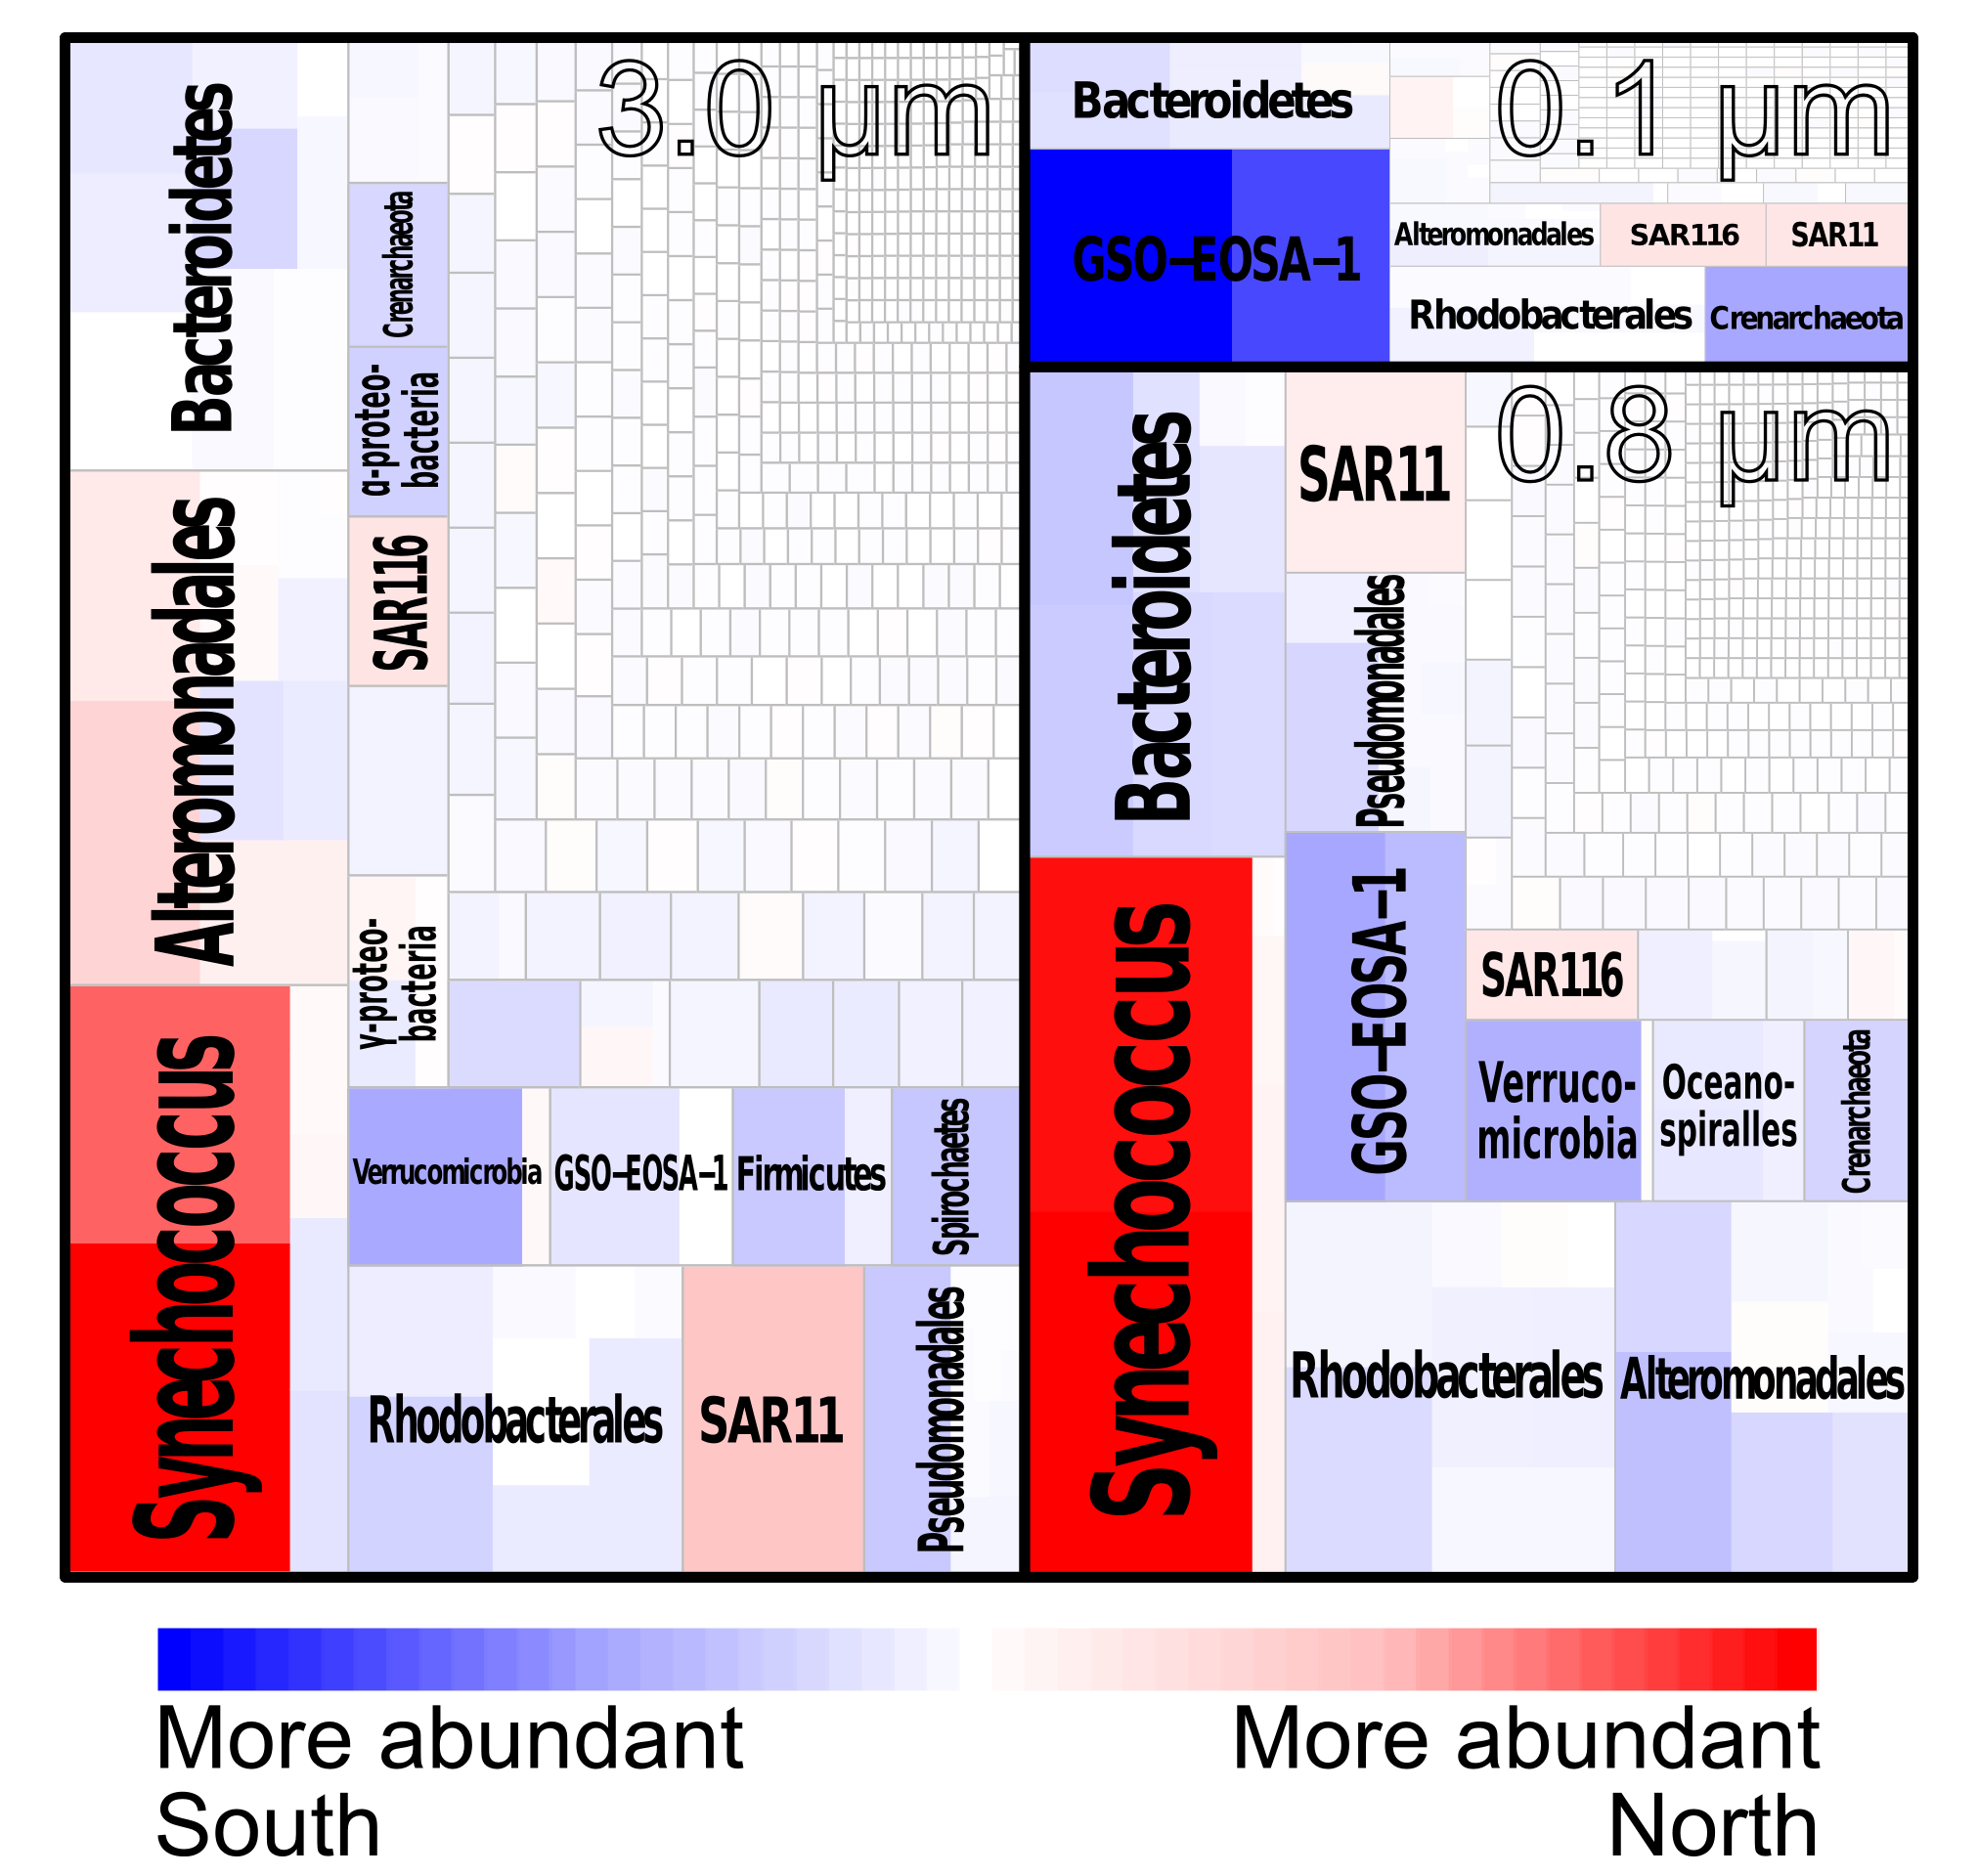
\includegraphics[width=\textwidth]{../polarfront/taxotreemap.png}
  \caption[Contribution of \acp{OTU} to variance between the North and South zones]{Contribution of \acp{OTU} to variance between the North and South zones, and differential abundance of \acp{OTU} from each size fraction between the two zones.
Each coloured (red or blue) rectangle represents an OTU identified through analysis of BLAST matches between SO metagenome data and the RefSeq database.
The area of each rectangle as a proportion of the total plot area corresponds to that \ac{OTU}'s contribution to the total variance between the two zones.
The colour of each rectangle corresponds to difference in relative abundance of that OTU between the zones, with blue indicating a higher relative abundance south of the PF, and red a higher abundance north of the PF.
\acp{OTU} from clades or taxonomic ranks of interest have been grouped, with labels in bold and groups separated by gray lines. 
Groups and \acp{OTU} with a low contribution to variance which were not grouped are unlabeled.
\acp{OTU} from each size fraction have also been grouped, with labels in black outline and size fractions separated by thick black lines. 
The data used to generate this figure are given in the supplementary material \suppfile{PF-OTUs-SIMPER.csv}.
  }
  \label{fig:taxotreemap}
\end{figure}


\ac{SIMPER} analysis found that no single \ac{OTU} contributed more than 2.9\% of variance, and 74\% of variance was contributed by \acp{OTU} with a contribution less than 1\%.
There was also a large difference in the contribution to variance of the three size fractions, with approximately 52\% of all variance contributed by \acp{OTU} from the 3.0 \micron{} fraction, 37\% by the 0.8 \micron{} fraction, and 9\% by the 0.1 \micron{} fraction.
Notably, \acp{OTU} within several taxonomic groups that had high contribution to variance covaried in their relative representation in the \ac{NZ} and \ac{SZ}.
For example, Bacteroidetes and GSO-EOSA-1 representatives were on average more abundant in the \ac{SZ}; while \genus{Prochlorococcus} and \genus{Synechococcus} species, SAR11 and SAR116 were on average more abundant in the \ac{NZ} \figref{fig:taxotreemap}.
Some groups, such as the Alteromonadales, had variable relative representation depending on size fraction.

\subsection{Fragment recruitment to verify \ac{OTU} identification}

As predicted, read recruitment to reference genomes produced fairly even coverage, especially in the high-abundance \acp{OTU}.
This indicates that \ac{OTU} identification was accurate and unlikely to be confounded by small regions of genomic identity.
\figreft{fig:frps} gives examples of read recruitment plots to three high-abundance and three low-abundance \acp{OTU}.

\afterpage{
  \centering
  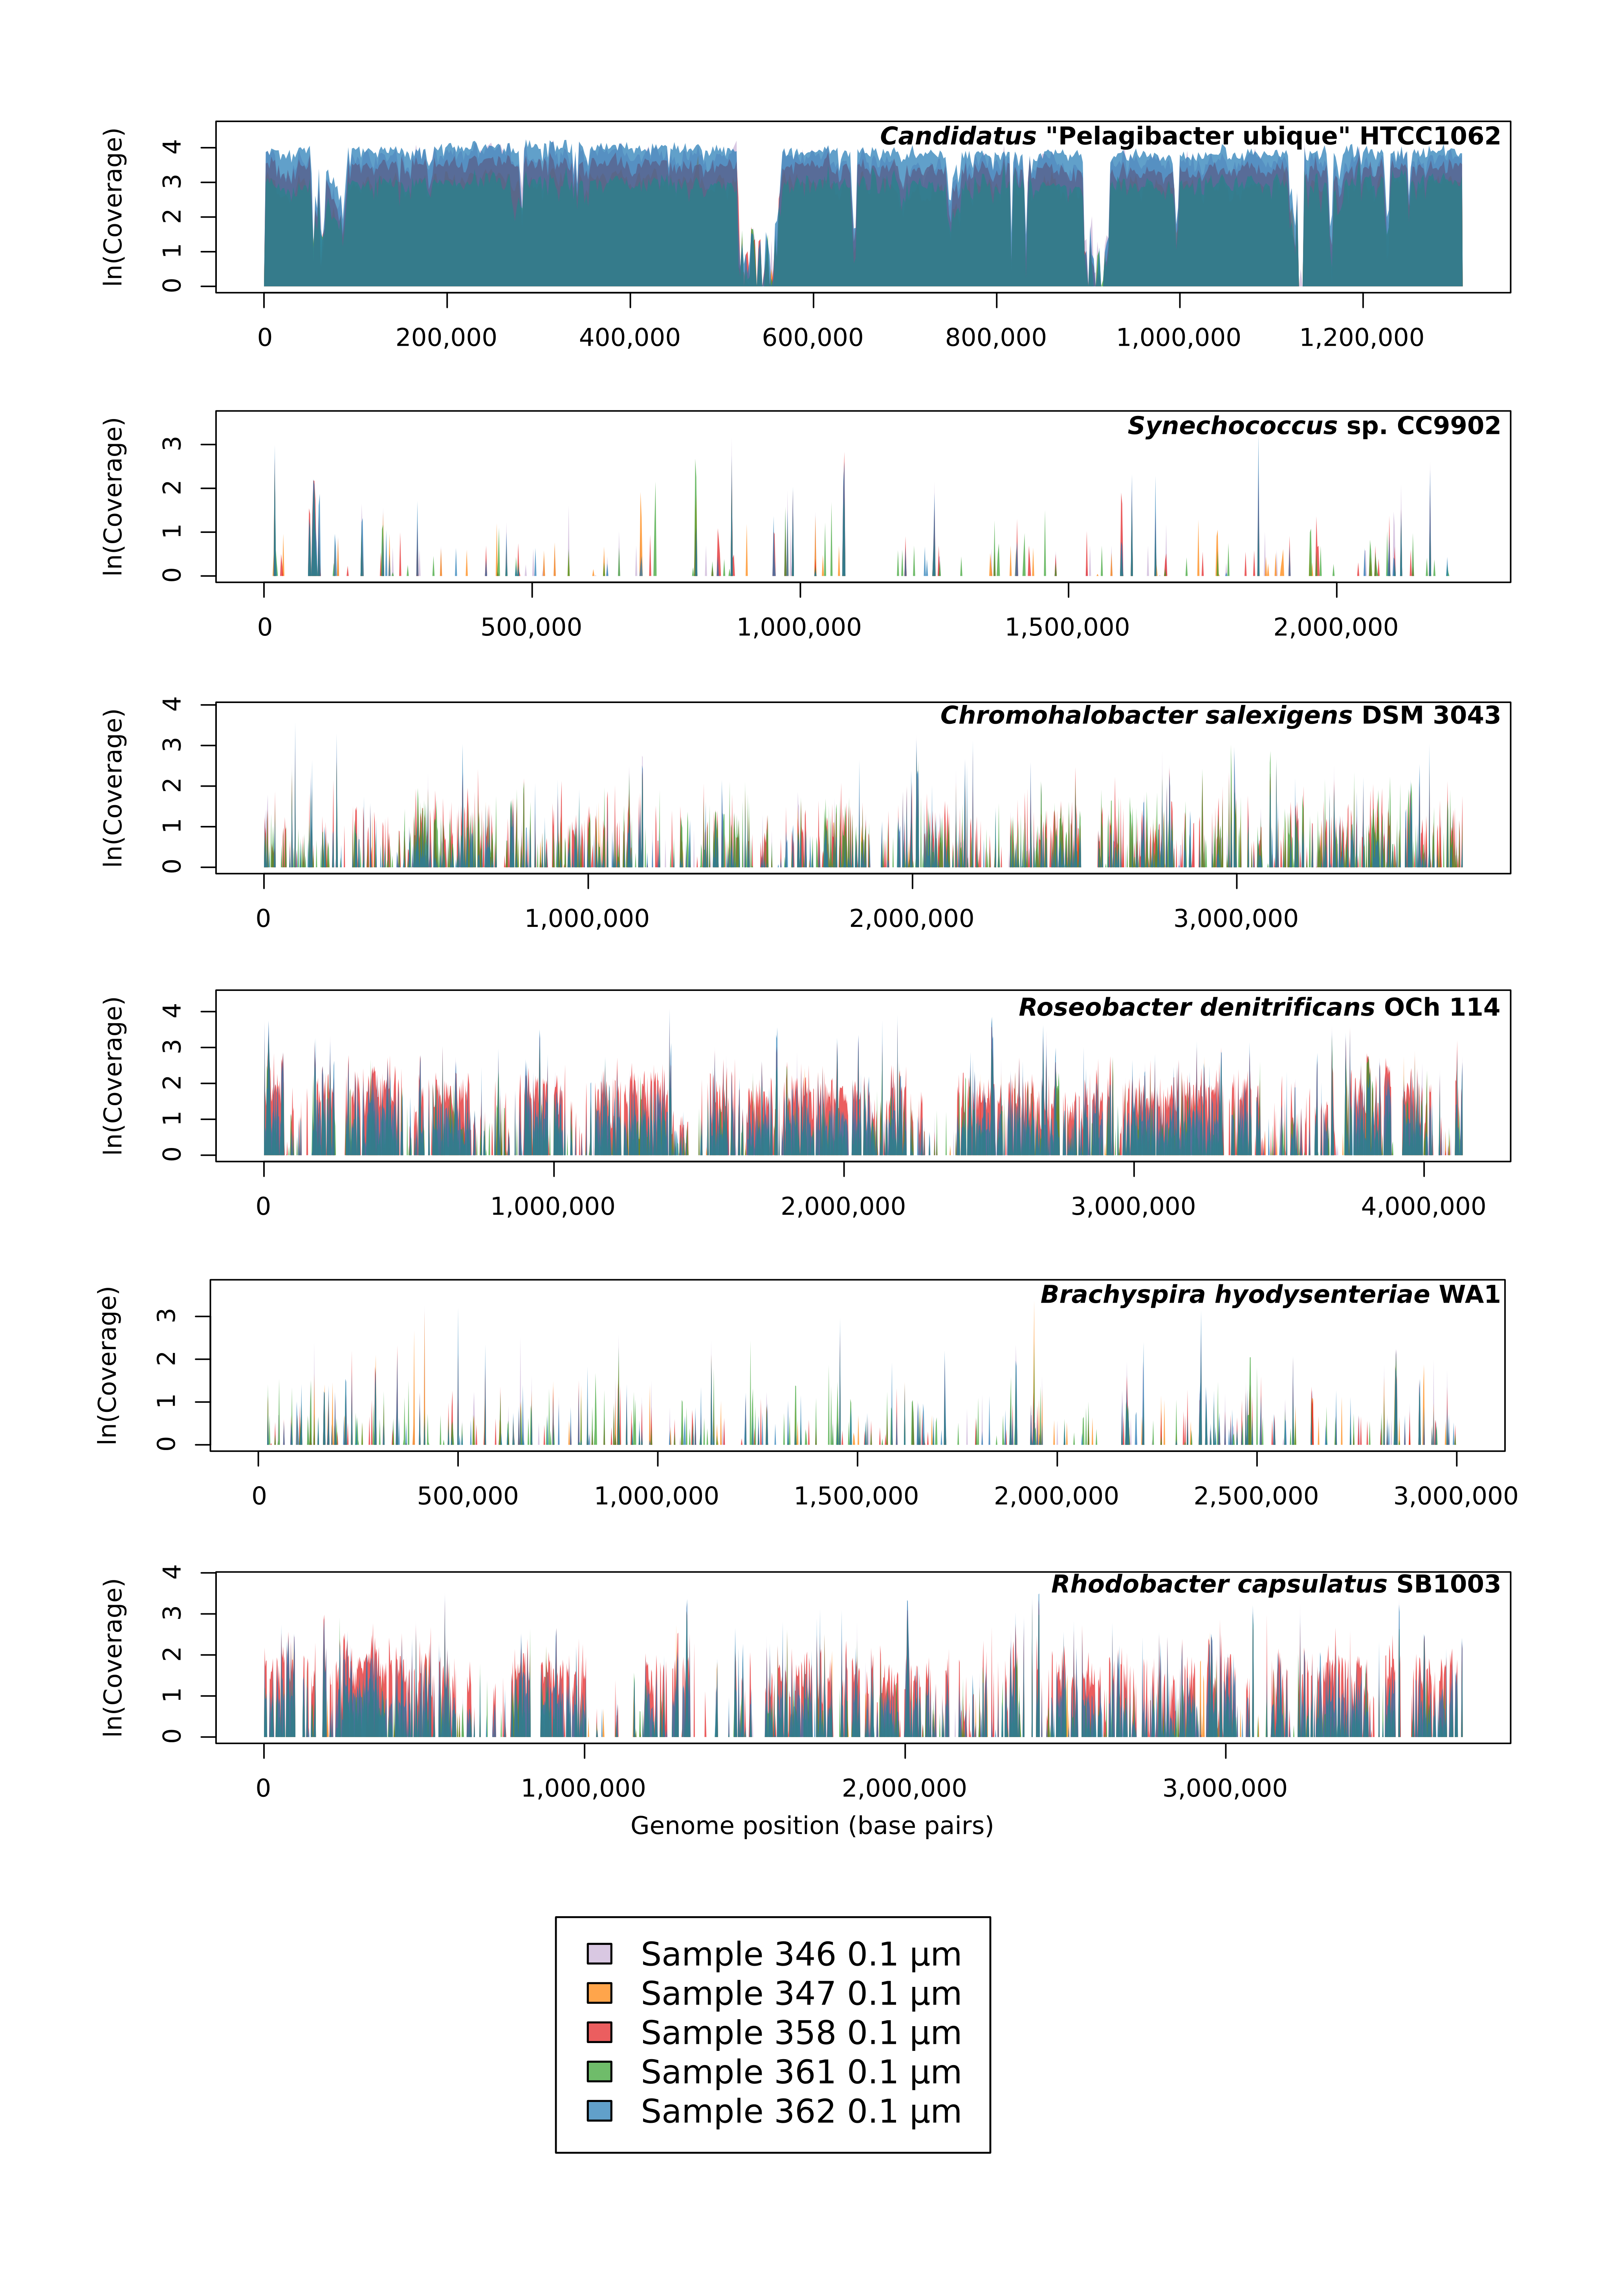
\includegraphics[height=\textheight]{../polarfront/frps.png}
  \captionof{figure}[Read recruitment to reference genomes]{\sffamily{}Examples of read recruitment (fragment recruitment) plots of metagenomic reads to reference genomes.
  The even distribution of recruitment sites across the genome suggests that \acp{OTU} identifications are relatively accurate; an \ac{OTU} identification resulting from a small region of genomic identity would generate a plot with read recruitment concentrated in small islands.
  \\
  \rule[1ex]{2cm}{0.5pt}
  }
  \label{fig:frps}
}


\subsection{Additional samples to test alternative ``polynya hypothesis''}
The \ac{ANOSIM} analysis strongly supported the ``\ac{PF} hypothesis'' (R = 0.44, p = 0.002), i.e.\ that the \ac{PF} was primarily responsible for the difference observed between the \ac{NZ} and \ac{SZ}, over the ``polynya hypothesis'' (R = 0.29, p = 0.005) that the influence of the Mertz Glacier polynya was responsible.
This also provides evidence that the \ac{PF} effect is robust over a longitudinal range and over time.

\subsection{Functional analysis of metagenomic data}

\ac{ANOSIM} analysis of the samples' \ac{KEGG} ortholog group and module profiles revealed that the zones had significantly different functional potential (ortholog group: R = 0.64, p = 0.001; module: R = 0.87, p = 0.001). 
\ac{SIMPER} was performed on the profiles in order to identify the specific functional differences between the zones. 
The highest-contributing modules are given in \tabreft{tab:modulessimper}, and a complete list in the supplementary material \suppfile{PF-modules-SIMPER.csv}.
The highest-contributing ortholog groups are given in \tabreft{tab:orthologsimper}, and a complete list in the supplementary material \suppfile{PF-ortholog-groups-SIMPER.csv}.
No single ortholog group or module contributed more than 2.2\% of the variance. 
There was a strong trend for ortholog groups and modules with higher contributions to variance to be overrepresented in the \ac{NZ} in the 3.0 \micron{} fraction but the \ac{SZ} in the smaller fractions, indicating that the functional diversity of each zone was strongly segregated by size fraction.

\begin{sidewaystable}
\sffamily
\begin{center}
\caption[Contributions of KEGG modules to variance between the North and South zones]{\sffamily{}The thirty \ac{KEGG} modules with the highest contributions to the difference between the \ac{NZ} and \ac{SZ}.
Abundances are zonal averages and have been standardised and log-transformed.
}
\label{tab:modulessimper}
\smallskip
\begin{tabularx}{\textwidth}{Xlll}
\toprule
\textbf{\ac{KEGG} module} & \textbf{Abundance} & \textbf{Abundance} & \textbf{Contribution to}\\
& \textbf{South} & \textbf{North} & \textbf{variance (\%)}\\
\midrule
Photosystem II & 0.42 & 0.57 & 2.21\\
Complex I (NADH dehydrogenase), NADH dehydrogenase I/diaphorase subunit of the bidirectional hydrogenase & 0.01 & 0.24 & 1.80\\
Photosystem I & 0.43 & 0.34 & 1.70\\
Pyrimidine deoxyribonucleotide biosynthesis, CDP/CTP \textrightarrow{} dCDP/dCTP,dTDP/dTTP & 0.51 & 0.66 & 1.16\\
Histidine degradation, histidine \textrightarrow{} N-formiminoglutamate \textrightarrow{} glutamate & 0.42 & 0.31 & 1.14\\
Methionine salvage pathway & 0.29 & 0.43 & 1.14\\
sn-Glycerol 3-phosphate transport system & 0.29 & 0.16 & 1.11\\
Complex I (NADH dehydrogenase), NADH dehydrogenase I & 1.08 & 1.05 & 1.06\\
Branched-chain amino acid transport system & 0.79 & 0.83 & 0.96\\
Dipeptide transport system & 0.14 & 0.02 & 0.95\\
Adenine nucleotide biosynthesis, IMP \textrightarrow{} ADP/dADP,ATP/dATP & 0.62 & 0.74 & 0.95\\
Glycine betaine/proline transport system & 0.66 & 0.56 & 0.94\\
Sulfur reduction, sulfate \textrightarrow{} H2S & 0.54 & 0.44 & 0.91\\
Simple sugar transport system & 0.46 & 0.39 & 0.90\\
Peptides/nickel transport system & 0.99 & 0.98 & 0.89\\
Ribosome, eukaryotes & 0.26 & 0.27 & 0.89\\
Multiple sugar transport system & 0.55 & 0.55 & 0.86\\
Type II general secretion system & 0.21 & 0.21 & 0.82\\
Sulfonate/nitrate/taurine transport system & 0.45 & 0.37 & 0.82\\
Guanine nucleotide biosynthesis, IMP \textrightarrow{} GDP/dGDP,GTP/dGTP & 0.72 & 0.82 & 0.81\\
RNA polymerase II, eukaryotes & 0.11 & 0.20 & 0.76\\
Histidine biosynthesis, PRPP \textrightarrow{} histidine & 0.94 & 0.86 & 0.76\\
Putrescine transport system & 0.18 & 0.09 & 0.72\\
Leucine biosynthesis, pyruvate \textrightarrow{} 2-oxoisovalerate \textrightarrow{} leucine & 1.29 & 1.37 & 0.71\\
C5 isoprenoid biosynthesis, non-mevalonate pathway & 0.70 & 0.77 & 0.71\\
Leucine degradation, leucine \textrightarrow{} acetoacetate + acetyl-CoA & 0.64 & 0.59 & 0.71\\
Thiamine transport system & 0.13 & 0.05 & 0.69\\
Spliceosome, 35S U5-snRNP & 0.18 & 0.20 & 0.68\\
Cytochrome b6f complex & 0.14 & 0.12 & 0.67\\
Menaquinone biosynthesis, chorismate \textrightarrow{} menaquinone & 0.25 & 0.27 & 0.66\\
\bottomrule
\end{tabularx}
\end{center}
\end{sidewaystable}

\begin{landscape}
\begin{table}
\sffamily
\begin{center}
\caption[Contributions of KEGG ortholog groups to variance between the North and South zones]{\sffamily{}
The thirty \ac{KEGG} ortholog groups with the highest contribution to the difference between the \ac{NZ} and \ac{SZ}.
Abundances are zonal averages and have been standardised and log-transformed.
As each ortholog group on each size fraction was encoded as a separate variable in the \ac{SIMPER} analysis, the size fraction is given after each ortholog group name.
}
\label{tab:orthologsimper}
\smallskip
\begin{tabularx}{\linewidth}{Xlll}
\toprule
\textbf{KEGG ortholog group} & \textbf{Abundance} & \textbf{Abundance} & \textbf{Contribution to}\\
& \textbf{South} & \textbf{North} & \textbf{variance (\%)}\\
\midrule
Hypothetical protein 3.0 \micron & 0.11 & 0.24 & 0.26\\
Hypothetical protein 0.8 \micron & 0.68 & 0.57 & 0.24\\
Ribonucleoside-diphosphate reductase alpha chain [EC:1.17.4.1] 0.8 \micron & 0.17 & 0.24 & 0.15\\
DNA polymerase III subunit alpha [EC:2.7.7.7] 0.8 \micron & 0.25 & 0.19 & 0.14\\
Hypothetical protein 0.1 \micron & 0.26 & 0.24 & 0.12\\
Proline dehydrogenase / delta 1-pyrroline-5-carboxylate 0.8 \micron & 0.10 & 0.04 & 0.12\\
Aminomethyltransferase [EC:2.1.2.10] 0.8 \micron & 0.25 & 0.19 & 0.12\\
Ribonucleoside-diphosphate reductase alpha chain [EC:1.17.4.1] 3.0 \micron & 0.02 & 0.08 & 0.12\\
Sarcosine oxidase, subunit alpha [EC:1.5.3.1] 0.8 \micron & 0.22 & 0.17 & 0.12\\
Integrator complex subunit 6 3.0 \micron & 0.07 & 0.05 & 0.11\\
Multicomponent Na$^{+}$:H$^{+}$ antiporter subunit D 0.8 \micron & 0.11 & 0.05 & 0.11\\
Glutamine synthetase [EC:6.3.1.2] 0.8 \micron & 0.24 & 0.19 & 0.11\\
Pyruvate dehydrogenase E1 component [EC:1.2.4.1] 0.8 \micron & 0.15 & 0.10 & 0.11\\
Cobaltochelatase CobN [EC:6.6.1.2] 0.8 \micron & 0.11 & 0.06 & 0.11\\
Formate dehydrogenase, alpha subunit [EC:1.2.1.2] 0.8 \micron & 0.15 & 0.10 & 0.11\\
DNA-directed RNA polymerase subunit beta [EC:2.7.7.6] 3.0 \micron & 0.03 & 0.08 & 0.11\\
Glutamate synthase (NADPH/NADH) large chain [EC:1.4.1.13 1.4.1.14] 0.8 \micron & 0.25 & 0.22 & 0.11\\
Dimethylglycine dehydrogenase [EC:1.5.99.2] 0.8 \micron & 0.17 & 0.14 & 0.11\\
Flagellin 0.8 \micron & 0.06 & 0.10 & 0.10\\
DNA-directed RNA polymerase subunit beta [EC:2.7.7.6] 3.0 \micron{}\footnote{Due to an error in the \ac{KEGG} database, this module is encoded twice.} & 0.03 & 0.08 & 0.10\\
Photosystem II PsbA protein 0.8 \micron & 0.01 & 0.06 & 0.09\\
Aldehyde dehydrogenase (NAD+) [EC:1.2.1.3] 0.8 \micron & 0.17 & 0.13 & 0.09\\
Glutamate synthase (NADPH/NADH) large chain [EC:1.4.1.13 1.4.1.14] 3.0 \micron & 0.02 & 0.07 & 0.09\\
Thymidylate synthase (FAD) [EC:2.1.1.148] 0.8 \micron & 0.02 & 0.06 & 0.09\\
Topoisomerase IV subunit A [EC:5.99.1.-] 0.8 \micron & 0.11 & 0.07 & 0.09\\
DNA mismatch repair protein MutS 0.8 \micron & 0.13 & 0.08 & 0.09\\
Glutamate dehydrogenase [EC:1.4.1.2] 0.8 \micron & 0.07 & 0.03 & 0.09\\
DNA polymerase I [EC:2.7.7.7] 0.1 \micron & 0.12 & 0.11 & 0.09\\
GTP-binding protein 0.8 \micron & 0.26 & 0.21 & 0.09\\
GTP-binding protein 3.0 \micron & 0.03 & 0.07 & 0.09\\
\bottomrule
\end{tabularx}
\end{center}
\end{table}
\end{landscape}


\section{Discussion}

\subsection{Taxonomic groups differentiating the zones}

\subsubsection{GSO-EOSA-1}

The \ac{GSO-EOSA-1} cluster, represented in RefSeq by \candidatus{Vesicomyosocius okutanii} strain HA and \candidatus{Ruthia magnifica} strain Cm. (\species{Calyptogena magnifica}) \cite{Walsh:2009fja}, made a large contribution to variance between the \ac{NZ} and \ac{SZ}, with higher abundance in the \ac{SZ}: relative abundances of \ac{GSO-EOSA-1} in the \ac{SZ} were 5.2\%, 3.4\% and 0.25\% in the 0.1, 0.8 and 3.0 \micron{} size fractions respectively, compared to 1.1\%, 0.84\% and 0.30\% in the \ac{NZ} \tabref{tab:topotus}.
The contribution to variance of this group was highest in the 0.1 \micron{} size fraction, followed by 0.8 \micron{} and 3.0 \micron{} \tabref{tab:otussimper}.
This pattern most likely represents a small cell size and lack of association with particulate matter.

\candidatus{Ruthia magnifica} and \candidatus{Vesicomyosocius okutanii} are chemoautotrophic endosymbionts of deep-sea bivalves \cite{Kuwahara:2007gf,Newton:2007fu} and are thus unlikely to be present in open ocean surface waters. 
However, \ac{GSO-EOSA-1} representative ARCTIC96BD-19 has recently been reported at high abundance in Antarctic coastal waters \cite{Ghiglione:2011ee,Grzymski:2012ej}.
To investigate the correct taxonomic placement of the \ac{GSO-EOSA-1} representative in this study, reads with identity to \candidatus{Ruthia magnifica} and \candidatus{Vesicomyosocius okutanii} were compared to the 16S rRNA gene of the SUP05 \ac{GSO-EOSA-1} isolate identified by \citet{Walsh:2009fja} (GenBank accession GQ351268.1) by \softwarename{blastn} with default settings and an E-value threshold of $10^{-3}$.
16S rRNA sequences from a reference set of endosymbiotic (\candidatus{Ruthia magnifica}, \candidatus{Vesicomyosocius okutanii}, \species{Solemya reidi} gill symbiont (GenBank accession L25709.1), \species{Bathymodiolus septemdierum} thioautotrophic gill symbiont (GenBank accession AB036709.1), \species{Vesicomya gigas} gill symbiont (GenBank accession AF035726.1) and \species{Ridgeia piscesae} endosymbiont (GenBank accession JX570608.1)) and planktonic (SUP05, ARCTIC96BD-19 (GenBank accession AF354606.1)) \ac{GSO-EOSA-1} representatives were obtained.
A neighbour-joining phylogenetic tree was constructed using \softwarename{ARB} \cite{Ludwig:2004dg}, using \species{Escherichia coli} IHE3034 (GenBank accession CP001969.1) as a gammaproteobacterial outgroup to root the tree.
The \ac{GSO-EOSA-1} 16S rRNA gene-affiliated metagenome reads were then placed in this tree by the ``\softwarename{ARB} parsimony'' insertion method, with alignments manually verified.
The majority of 16S rRNA genes from all samples and size fractions clustered with ARTIC96BD-19 \figref{fig:GSO-EOSA-1tree}, indicating this is the dominant GSO-EOSA-1 representative. 

\begin{figure}[!ht]
  \centering
  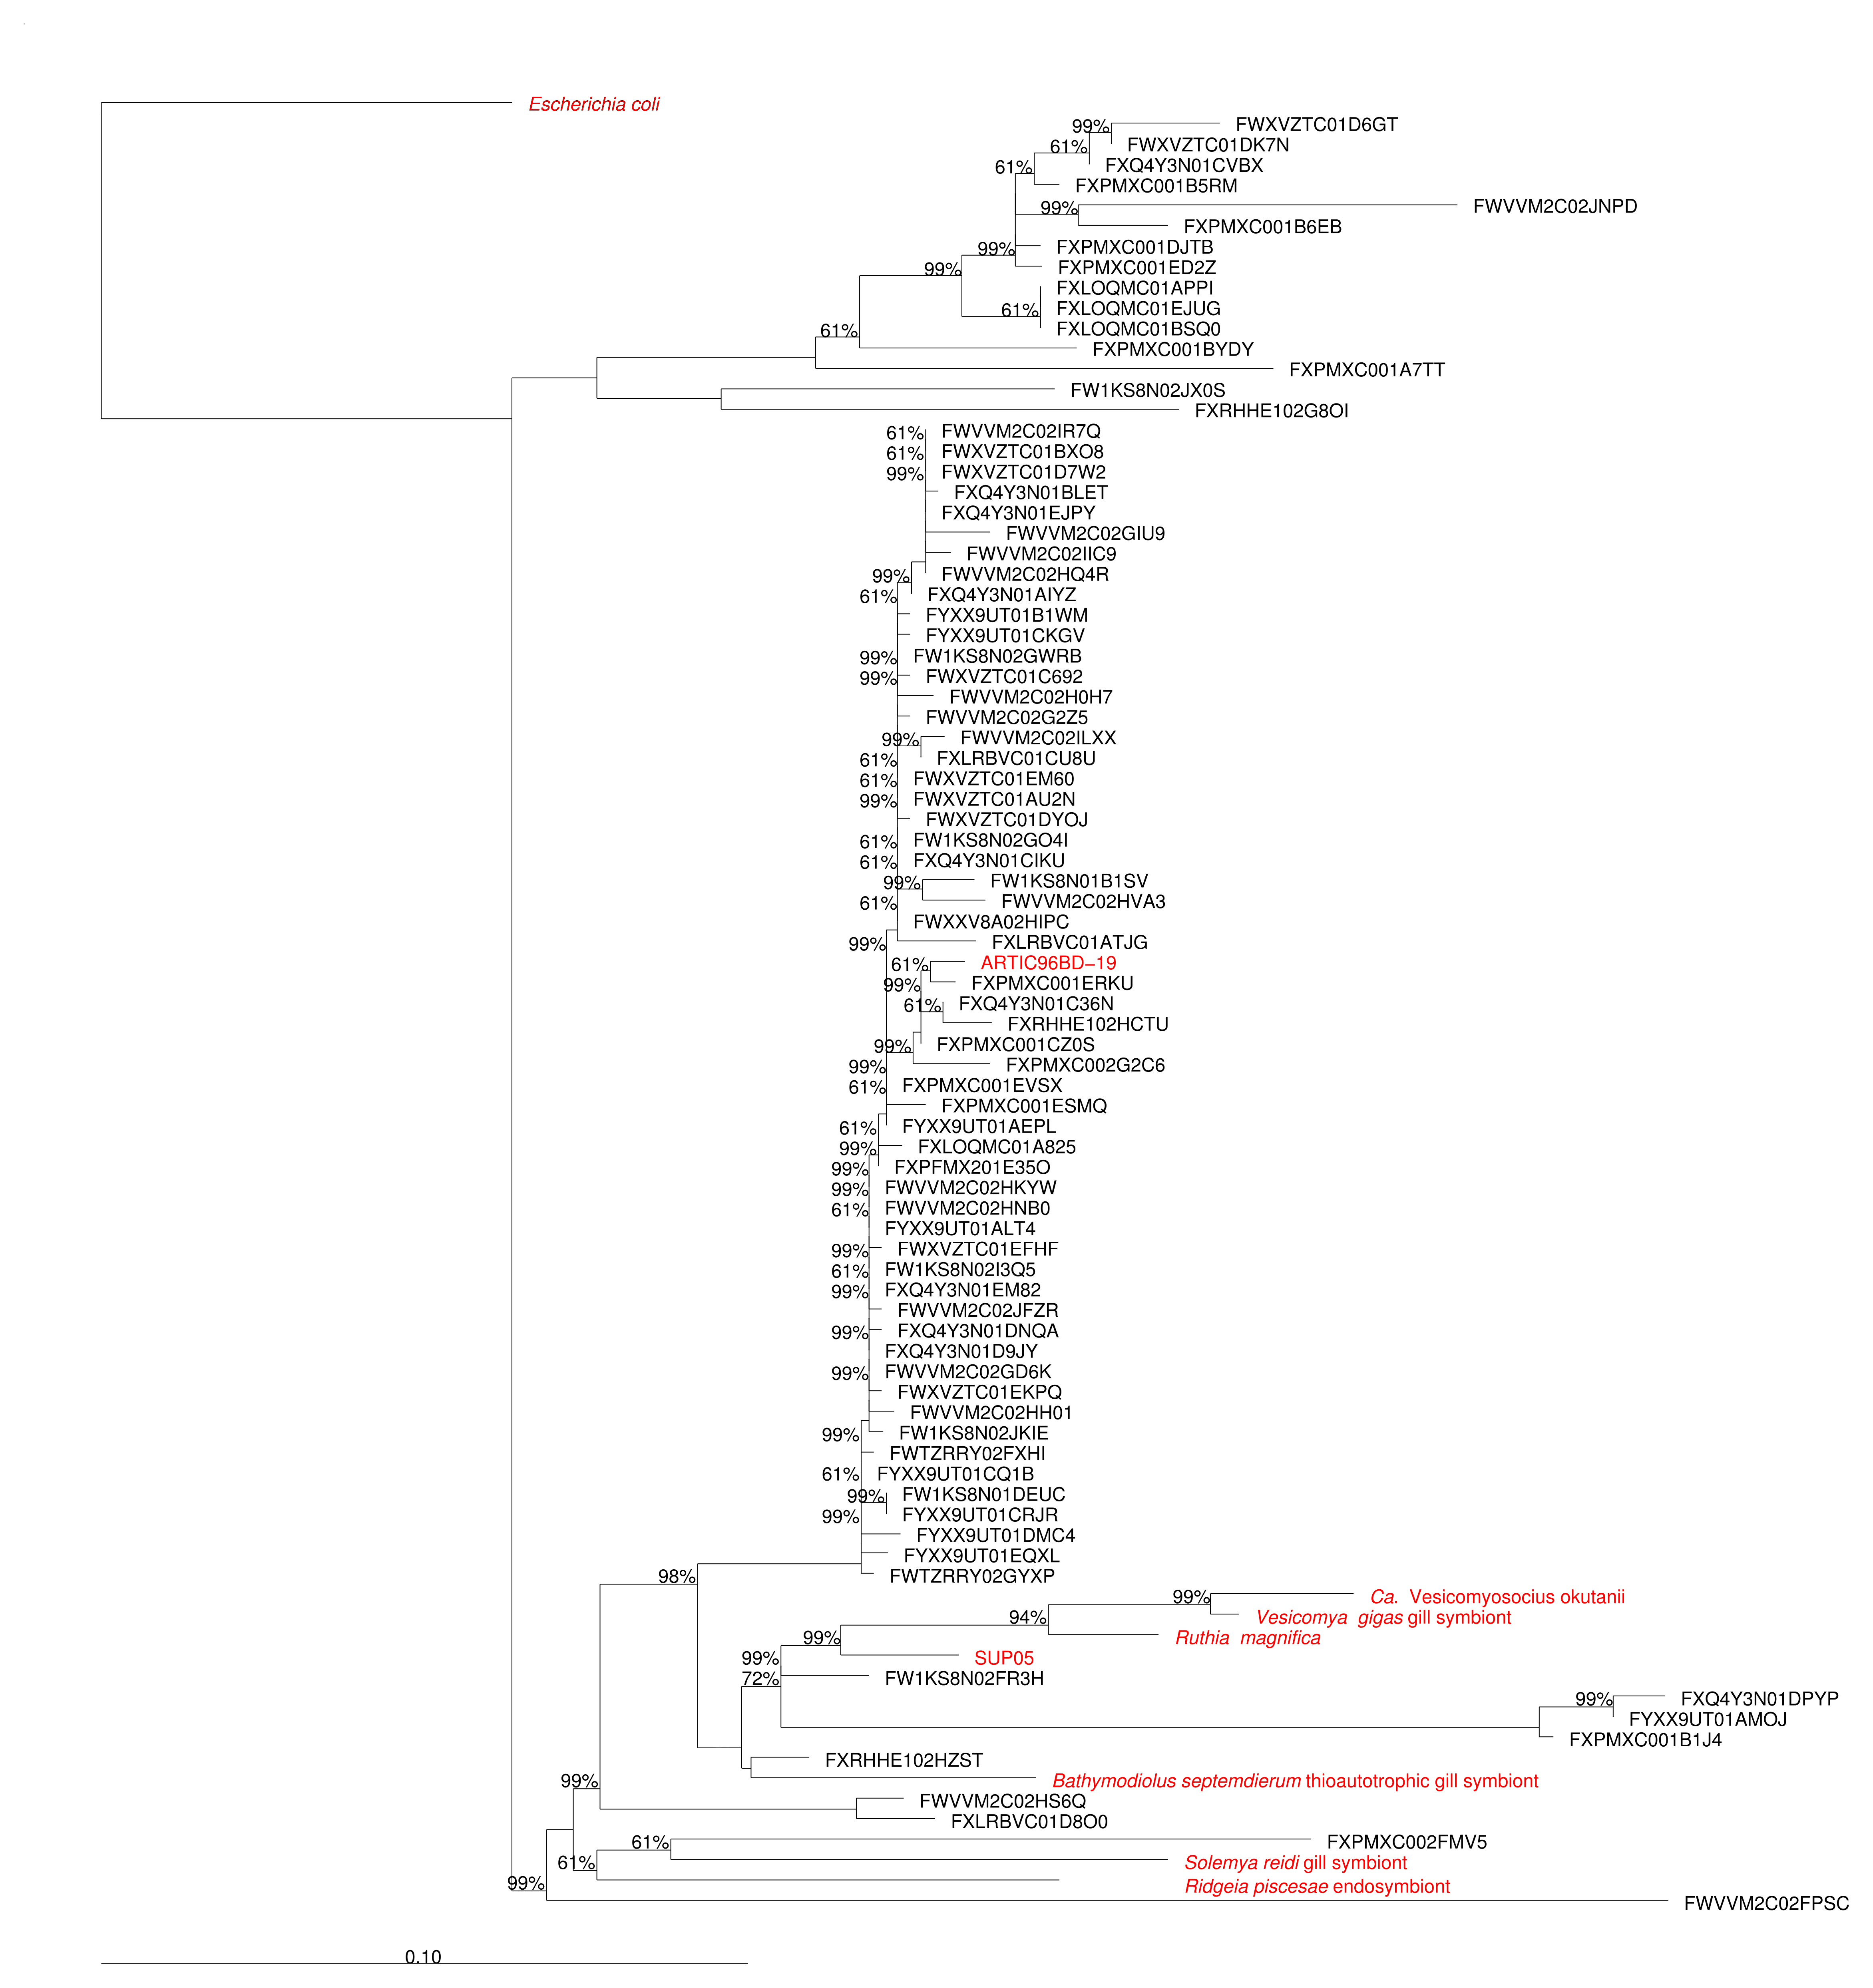
\includegraphics[width=\textwidth]{../polarfront/GSO-EOSA-1tree.png}
  \caption[Tree of GSO-EOSA-1 related 16S rRNA genes]{
  Neighbour-joining tree of GSO-EOSA-1-like 16S rRNA gene sequences from the metagenomes in this study.
  Sequences labeled in black text are reads from the metagenomes.
  Red labels are 16S rRNA gene sequences from Gammaproteobacterial Sulfur Oxidizers (GSO) and other Gammaproteobacteria.
  Bootstrap values for each node are indicated as percentages.
  The tree was constructed using \softwarename{arb} \cite{Ludwig:2004dg}.
  }
  \label{fig:GSO-EOSA-1tree}
\end{figure}
\clearpage


Single-cell genomic analysis of ARCTIC96BD-19 from global mesopelagic waters indicates the lineage is probably mixotrophic, able to couple carbon fixation to oxidation of reduced sulphur compounds as well as assimilate organic carbon \cite{Swan:2011hb}.
\ac{GSO-EOSA-1} cytochrome C oxidase (CoxII) has been identified in a winter metaproteome of Antarctic Peninsula coastal waters, suggesting the capacity for aerobic respiration \cite{Williams:2012bs}.
Taken together, this evidence suggests the \ac{GSO-EOSA-1} representative in Antarctic coastal waters is a versatile chemolithoautotroph capable of aerobic respiration.

It has been proposed that during the winter months, chemolithoautotrophy is dominant over photoautotrophy as the major carbon fixation process in \ac{AZ} waters due to the lack of available light, both from seasonal darkness and ice shading \cite{Grzymski:2012ej}.
The high relative abundance of \ac{GSO-EOSA-1} in \ac{SZ} compared to \ac{NZ} waters may therefore represent the remnants of an annual winter increase in population in the marginal ice zone which does not occur in the open ocean.

\subsubsection{Ammonia-oxidizing Crenarchaeota}

\species{Nitrosopumilus maritimus} SCM1 and \species{Cenarchaeum symbiosum} are chemolithoautotrophic, nitrifying members of the \ac{MGI} \cite{Preston:1996vi,Walker:2010ww}.
These species were the only representatives in the reference database used in this study of the \ac{AOA}.
The contribution of \species{Cenarchaeum symbiosum} to total \ac{AOA} abundance was low (0--0.015\% across all fractions and zones, \suppfile{PF-all-OTUs.txt}).
As \species{Cenarchaeum symbiosum} is a sponge symbiont \cite{Preston:1996vi} and given the poor representation of \ac{AOA} in RefSeq, it is likely this \ac{OTU} has attracted sequences originating from planktonic \ac{AOA} and \species{Cenarchaeum symbiosum} itself is not present.
\ac{AOA} were moderate contributors to variance between the \ac{NZ} and \ac{SZ}, and were overrepresented in the \ac{SZ} in all size fractions \figref{fig:taxotreemap}.
As with the GSO-EOSA-1 cluster, \ac{MGI} have been proposed to be abundant chemolithoautotrophs and therefore major drivers of winter carbon fixation in Antarctic coastal waters \cite{Grzymski:2012ej,Williams:2012bs}.

Sample 353 had a particularly high relative abundance of \species{Nitrosopumilus maritimus} \acp{OTU} (7.5\% of the 0.1 \micron{} fraction; 0.8 \micron: 11\%; 3.0 \micron: 12\%).
This sample was taken closer to the Antarctic continent (3.7 km) than any other, in relatively shallow (180 m) waters 17.6 km from the Mertz Glacier.
The high abundance of ammonia oxidizers may reflect an input of ammonia from terrestrial sources (e.g.\ penguin guano), or resuspension of benthic sediments in which \ac{MGI} are abundant \cite{Bowman:2003fa} by near-shore turbulence and iceberg scouring.
Breakdown of water column stratification has been previously suggested as a cause of increased \ac{AOA} abundance in Antarctic coastal surface waters \cite{Kalanetra:2009bv}.

\subsubsection{Cyanobacteria}

\acp{OTU} assigned to the cyanobacterial genera \genus{Prochlorococcus} and \genus{Synechococcus} were overrepresented in the \ac{NZ} in all size fractions \figref{fig:taxotreemap}.
The mean relative abundance of cyanobacteria in samples 367 and 368, the two northernmost samples, was strikingly higher than the mean abundance across all other samples in the \ac{NZ}.
\genus{Synechococcus} sp. CC9902 alone composed greater than 22\% of the 0.8 \micron{} fraction in these samples, consistent with \genus{Synechococcus} species' cell diameters of up to 0.9 \micron \cite{Waterbury:1985js}.
The high abundance of both cyanobacterial genera on the 3.0 \micron{} fraction has previously been reported \cite{Lauro:2010jna} and may be attributable to aggregation \cite{Lomas:2011bp}.

Samples 367 and 368 were separated from the other samples north of the \ac{PF} by the \ac{STF}.
While the \ac{STF} was not a significant boundary on the assemblage level (ANOSIM, p > 0.05), it may mark a significant biogeographic boundary for these cyanobacteria.
\genus{Synechococcus} and \genus{Prochlorococcus} together represent a large proportion of both phytoplankton abundance and carbon fixation in temperate and tropical waters, in many regions contributing more than half of total primary production \cite{Liu:1997ub,Liu:1998tk,Andre:1999uh}.
The role of the \ac{STF} in determining the latitudinal range of \genus{Synechococcus} and \genus{Prochlorococcus} is therefore important, as it will affect models of ocean productivity under climate change, and warrants further investigation.
Despite the high abundance of cyanobacteria north of the \ac{STF}, they were also a significant feature of the \ac{SAZ}; for example, \genus{Synechococcus} sp. CC9902 composed 3--5\% of the 0.8 \micron{} fraction in \ac{SAZ} samples.

These results confirm previous reports \cite{Marchant:1987wv,Ghiglione:2011ee} that cyanobacteria occur as far south as the Antarctic coast, albeit at very low abundances (10\textsuperscript{3}--10\textsuperscript{4} cells/L \cite{Marchant:1987wv}), and contradicts the assumption that \genus{Prochlorococcus} is restricted to tropical and subtropical waters within 40\textdegree{} of latitude \cite{Partensky:1999uf}.
Cyanophage proteins have also been detected in a metaproteomic analysis of Antarctic Peninsula coastal surface waters \cite{Williams:2012bs}.

\subsubsection{SAR11 and SAR116 clades}

\candidatus{Pelagibacter ubique} HTCC1062 is a good representative of total SAR11 abundance in this study, as it is a member of the SAR11 phylotype which is most abundant in \ac{SO} waters \cite{Brown:2012gna}.
\candidatus{Pelagibacter ubique} HTCC1062 was the most abundant \ac{OTU} across all samples and fractions (\ac{NZ} average: 62\%, 25\% and 24\% of the 0.1 \micron{}, 0.8 \micron{} and 3.0 \micron{} fractions respectively; \ac{SZ}: 59\%, 22\% and 18\%) and one of the most significant contributors to variance between the \ac{NZ} and \ac{SZ}.
The high abundance of SAR11 in the 0.1 \micron{} fraction is consistent with the small size of SAR11 cells \cite{Rappe:2002wz}.
The higher representation in the \ac{NZ} may reflect the competitiveness of SAR11 members in regions with low \ac{DOC} concentrations due to low primary productivity \cite{Giovannoni:2005ib,Alonso:2006dj}, such as the \ac{HNLC} \ac{SAZ}.
Overall, these findings are consistent with reports that SAR11 is ubiquitous in the world's oceans \cite{Mary:2006wk,Carlson:2009cc} and more abundant north of the \ac{ACC} \cite{Giebel:2009hr}.

\acp{OTU} of \candidatus{Puniceispirillum marinum} from the SAR116 clade were a moderate contributor to variance between the \ac{NZ} and \ac{SZ} with higher abundance in the \ac{NZ} \figref{fig:taxotreemap}.
A genomic analysis reported \candidatus{Puniceispirillum marinum} IMCC1322 to be a metabolic generalist with genes for aerobic CO fixation, C1 metabolism and a \candidatus{Pelagibacter ubique}-like \ac{DMSP} demethylase, suggesting SAR116 and SAR11 occupy similar ecological niches \cite{Oh:2010di}.
In the Scotia Sea, SAR116 abundance (determined using \ac{FISH}) was reported to be higher in more productive waters where SAR11 numbers were lower \cite{Topping:2006ul}.
However, this analysis across an extended latitudinal transect indicates that overall SAR11 and SAR116 have similar biogeographic distributions.

\subsubsection{Bacteroidetes}

\acp{OTU} of the phylum Bacteroidetes, in particular members of the class Flavobacteria, were found to be abundant (\ac{NZ} average: 1.2\%, 5.0\% and 6.9\% of the 0.1 \micron{}, 0.8 \micron{} and 3.0 \micron{} fractions respectively; SZ: 2.3\%, 9.8\% and 9.1\%) and significant contributors to variance between the \ac{NZ} and \ac{SZ} \figref{fig:taxotreemap}.
Flavobacteria have been previously reported to compose the majority of both Bacteroidetes \cite{Murray:2007db} and total planktonic biomass \cite{Abell:2005ji} in the \ac{SO}, as well as being abundant in sea ice \cite{Brown:2001hh}.
As heterotrophic degraders of \ac{HMW} compounds in the form of both \ac{DOM} and \ac{POM} \cite{Kirchman:2002ub}, marine Flavobacteria are major components of marine aggregates \cite{Rath:1998wm,Crump:1999wo,Zhang:2007fb}.
The higher abundance of Flavobacteria \acp{OTU} on the 0.8 \micron{} and 3.0 \micron{} fractions indicates their association with particulate matter.
Similar size partitioning of \ac{SO} Flavobacteria has previously been reported \cite{Abell:2005ji}.

The higher abundance of \acp{OTU} of Flavobacteria in the \ac{SZ} may reflect an input of cells from melting sea ice \cite{Brown:2001hh}, the higher rates of primary productivity in the south, and the role of the Flavobacteria as degraders of \ac{HMW} \ac{DOM}.
Because deposition of marine snow is a major route for sequestration of fixed carbon in the ocean \citep[e.g.][]{Hessen:2004vq}, the Flavobacteria that associate with this particulate matter represent a remineralising shunt, which would decrease carbon sequestration by this route.

\subsubsection{Rhodobacterales}

Members of the order Rhodobacterales were abundant (\ac{NZ} average: 1.2\%, 10\% and 5.5\% of the 0.1 \micron{}, 0.8 \micron{} and 3.0 \micron{} fractions respectively; \ac{SZ}: 1.6\%, 13\% and 7.9\%) and high contributors to variance, overrepresented in the \ac{SZ} on all size fractions.
As several members of the Roseobacter clade have been shown to have symbiotic relationships with marine eukaryotic algae \cite{Buchan:2005hd,WagnerDobler:2006kb}, and their abundance in the \ac{SO} has previously been linked to phytoplankton blooms \cite{West:2008kc,Obernosterer:2011df}, it is likely that their overrepresentation in the \ac{SZ} is related to the higher density of phytoplankton in the \ac{AZ}.

\acp{OTU} of \species{Roseobacter denitrificans} Och114 and \species{Silicibacter pomeroyi} DSS-3 were consistently the most abundant Roseobacter clade representatives.
\species{Roseobacter denitrificans} and \species{Silicibacter pomeroyi} fall within a subclade of \ac{AAP} members of the Roseobacter clade \cite{Swingley:2007dm}.
These species have diverse mixotrophic metabolisms, with genomic and experimental evidence of photoheterotrophic respiration of organic carbon, fixation of \ce{CO_{2}}, oxidation of CO, oxidation of reduced sulfur compounds, and utilization of the abundant marine osmolyte \ac{DMSP} \cite{King:2003kc,Moran:2004ie,WagnerDobler:2006kb,Swingley:2007dm,Brinkhoff:2008do,Howard:2008hf}.
This metabolic diversity suggests a complex ecological role, particularly with respect to the capture and release of climatically active gases (\ce{CO_{2}}, CO, dimethylsulfide) involved in carbon and sulfur cycling.

\subsubsection{Alteromonadales}

Members of the gammaproteobacterial order Alteromonadales were large contributors to variance.
Most \acp{OTU} were overrepresented in the \ac{SZ} but some were overrepresented in the \ac{NZ} on the 3.0 \micron{} fraction \figref{fig:taxotreemap}.
\species{Colwellia psychrerythraea} 34H was one of the most abundant \acp{OTU} in the Alteromonadales that exhibited this distribution (\ac{NZ} average: 0.14\%, 2.2\% and 16\% of the 0.1 \micron{}, 0.8 \micron{} and 3.0 \micron{} fractions respectively; \ac{SZ}: 0.52\%, 5.1\% and 10\%).
\species{Colwellia psychrerythraea} 34H was isolated from Arctic sediment, grows well at low temperatures and secretes extracellular polysaccharides \cite{Huston:2000jr,Junge:2003kb,Methe:2005uf}.
Similar to other \genus{Colwellia} species grown under laboratory conditions, cells have widths of 0.4--0.8 \micron{} and lengths of 1.5--4.5 \micron{} \cite{Jung:2006fh}.
Growth temperature can have a major impact on cell morphology, enzyme secretion and global gene expression in psychrophiles \citep[e.g.][]{Feller:2003ir,Junge:2003kb,Williams:2011hy,Cavicchioli:2006bl,Campanaro:2011gj}.
Moreover, marine bacteria can alter their cell dimensions in response to nutrient flux \citep[e.g.][]{Kjelleberg:1987wp}.
It is therefore possible that the populations of Alteromonadales captured on the 3.0 \micron{} filters (overrepresented in the \ac{NZ}) had different physiological properties to those on the 0.1 and 0.8 \micron{} filters (overrepresented in the \ac{SZ}).

\subsubsection{Verrucomicrobia}

Two representatives of the phylum Verrucomicrobia, \species{Coraliomargarita akajimensis} and \genus{Akkermansia} sp. Muc-30, were moderate contributors to variance and overrepresented in the \ac{SZ} \figref{fig:taxotreemap}.
Surprisingly given the small cell size of \species{Coraliomargarita akajimensis} \cite{Yoon:2007ic}, its contribution to variance increased with size fraction.
A global survey reported a similar fractionation pattern, and suggested marine Verrucomicrobia may be predominantly particle attached \cite{Freitas:2012jz}.
However, little else is known about the distribution and ecological roles of marine Verrucomicrobia \cite{Freitas:2012jz}.

\subsection{Functional capacities differentiating the zones}

A number of modules with transport functions (sn-glycerol 3-phosphate transport system, dipeptide transport system, peptides/nickel transport system, simple sugar transport system, sulfonate/nitrate/taurine transport system) were overrepresented in the \ac{SZ} \tabref{tab:modulessimper}.
As the genomes of copiotrophic bacteria have evolved to have a higher number of narrow-specificity transporters relative to oligotrophic genomes \cite{Lauro:2009gx}, these differences may reflect the higher nutrient availability and thus a dominance of copiotrophs in the \ac{SZ}.
The taxonomic contributors to these modules were varied, although members of the Rhodobacterales were prominent \figref{fig:moduledecomp}.

\afterpage{
  \centering
  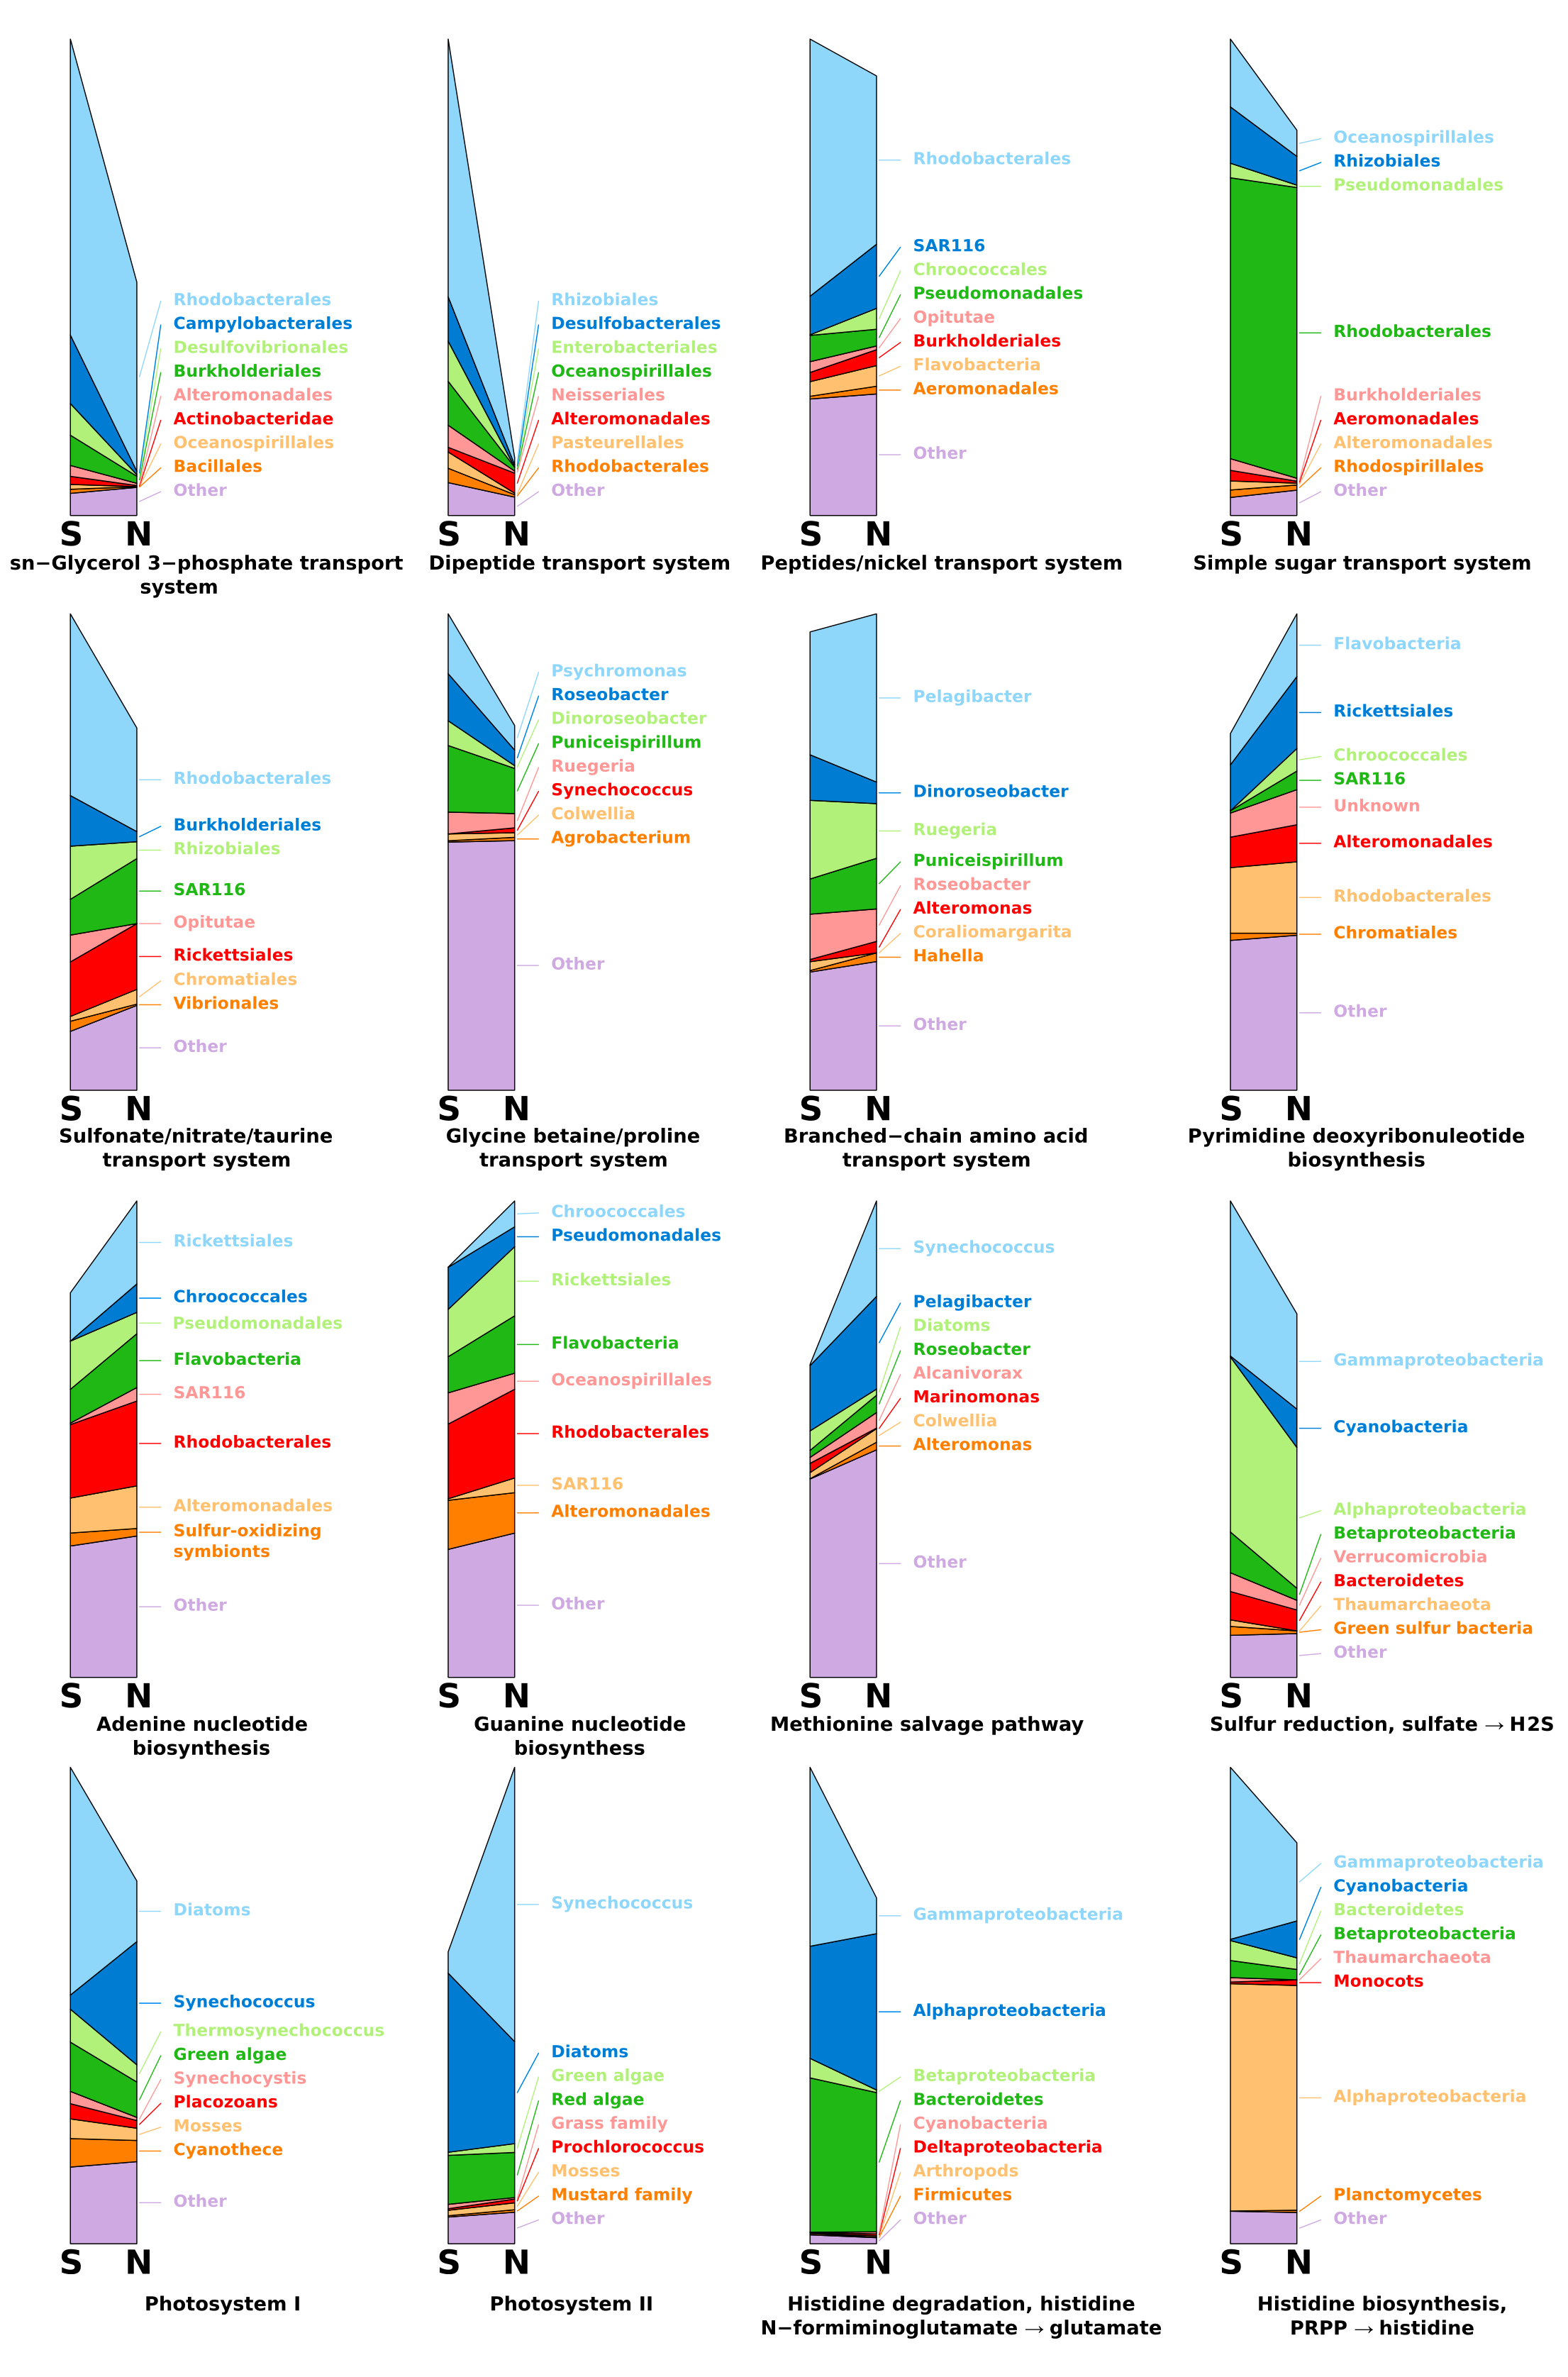
\includegraphics[width=\textwidth]{../polarfront/moduledecomp.png}
  \captionof{figure}[Taxonomic decomposition of KEGG modules]{Decomposition of KEGG modules of interest to contributing classes, orders or genera. The left side of each stack (S) indicates the proportion of the module abundance contributed by each class, order or genus in the South Zone, while the right side (N) represents the North Zone. As the contributions are relative and represent unitless module abundances, no axis is given and proportions are not comparable between modules. Contributing classes, orders or genera are arranged in descending order of the difference in the relative contributions between the zones. Only the eight highest contributors for each module are shown, with the remainder collapsed into the ``Other'' group. The taxonomic ranks to which each module was decomposed are as follows: sn-glycerol 3-phosphate transport, peptide-nickel transport, simple sugar transport and sulfonate/nitrate/taurine transport were decomposed to order; glycine betaine/proline transport and branched-chain amino acid transport to genus; pyrimidine deoxyribonucleotide biosynthesis, adenine nucleotide biosynthesis and guanine nucleotide biosynthesis to order; methionine salvage to genus; sulphur reduction to class; photosystem I and photosystem II to genus; histidine degradation to glutamate and histidine biosynthesis to class.\\
  \rule[1ex]{2cm}{0.5pt}
  }
  \label{fig:moduledecomp}
}


The glycine betaine/proline transport module was also overrepresented in the \ac{SZ}, though this probably reflects glycine betaine's role as an osmo- and cryoprotectant in the colder \ac{SZ} waters.
This is supported by the major taxonomic contributor to this module, genus \genus{Psychromonas}, which includes several psychrophilic species. 

One exception to this pattern was the branched-chain amino acid transport system module, overrepresented in the \ac{NZ}. 
The genera \genus{Pelagibacter} and \genus{Puniceispirillum} were major contributors to this module's overabundance in the \ac{NZ} \figref{fig:moduledecomp}.
As both SAR11 \cite{Giovannoni:2005ib} and SAR116 \cite{Grote:2011dm} representatives encode branched-chain amino acid transporters, the abundance of this module is likely to represent taxonomic differences between the zones.

Biosynthesis pathways for all major nucleic acids (pyrimidine deoxyribonucleotide biosynthesis, adenine nucleotide biosynthesis, guanine nucleotide biosynthesis) were consistently high contributors to variance and overabundant in the \ac{NZ}.
This pattern seems inconsistent with the more oligotrophic nature of the \ac{NZ}, as oligotrophic cells generally have smaller genomes \cite{Lauro:2009gx} and slower growth rates than copiotrophs, and would therefore be expected to require a lower rate of de novo nucleotide biosynthesis.
A possible explanation for this is that \ac{SZ} cells have higher availability of extracellular DNA as a byproduct of decaying phytoplankton \cite{Lomas:2011bp}, which can be imported and salvaged for nucleic acids \cite{Paul:1988wn} thus reducing the requirement for de novo synthesis.
No single taxonomic group contributed a large fraction of the difference in this module \figref{fig:moduledecomp}, suggesting this is a widespread adaptation.

The methionine salvage pathway module had a large contribution to variance between the zones and was overrepresented north of the \ac{PF}.
This may reflect the higher availability of \ac{DMSP} in the \ac{SZ} as a byproduct of blooming eukaryotic algae.
\ac{DMSP} is a major carbon and sulfur source for marine microorganisms, and is commonly assimilated by bacteria through demethylation to \ac{MMPA}, followed by further catabolism to the climatically important compounds dimethylsulfide or methanethiol \citep[review in][]{Curson:2011ic}.
However, when \ac{DMSP} is scarce, \ac{MMPA} may be derived from methionine through the alternative methionine salvage pathway \cite{Reisch:2012bb}.
The genus \genus{Synechococcus}, a noted contributor to marine \ac{DMSP} uptake and assimilation \cite{VilaCosta:2006gt}, was a very high contributor to the abundance of this module in the \ac{NZ} \figref{fig:moduledecomp}, suggesting \genus{Synechococcus} species may use this route when \ac{DMSP} is unavailable.

The sulfur reduction module was overrepresented in the \ac{SZ}, and it is likely that this result is strongly driven by taxonomic differences.
While the taxonomic breakdown indicated a large number of genera contributed to the difference, the Gammaproteobacteria were the highest-contributing class \figref{fig:moduledecomp}.
This module also includes the assimilatory sulfate reduction pathway, which is widespread in marine bacteria, but is absent from SAR11, with known representatives reported to lack genes for assimilatory sulfate reduction (cysDNCHIJ) \cite{Tripp:2008dd}.
The higher relative abundance of SAR11 in the \ac{NZ} may therefore contribute to the lower abundance of genes for assimilatory sulfate reduction in that zone. 

The sulfur reduction module also included adenylylsulfate reductase (APS reductase, encoded by aprAB), an enzyme implicated in sulfite detoxification during heterotrophic growth on organosulfonates \cite{Meyer:2007jd} (N.B. in recent \ac{KEGG} releases, aprA is no longer included in this module).
As the GSO-EOSA-1 representative SUP05 has been found to encode APS reductase, the overabundance of this module may reflect sulfur oxidation through the reverse dissimilatory sulfate reduction pathway \cite{Walsh:2009fja}.
Also, Roseobacter clade bacteria are involved in the decomposition of abundant organic sulfur compounds (e.g.\ \ac{DMSP}, organosulfonates), and hence have been accorded an important role in marine sulfur cycling \cite{Moran:2007fs}.

The photosystem II module was overrepresented in the \ac{NZ}.
Given the underrepresentation of cyanobacterial \acp{OTU} in the \ac{SZ}, this may reflect a dominance of primary production by eukaryotic algae south of the \ac{PF} and cyanobacteria to the north.
Decomposition of the taxonomic affiliations of ortholog groups contributing to this module found \acp{OTU} of \genus{Synechococcus} and \genus{Prochlorococcus} to be major contributors to the difference \figref{fig:moduledecomp}.
Variation in the photosystem I module, which was marginally overrepresented in the \ac{SZ}, could largely be attributed to diatoms and other eukaryotic phytoplankton \figref{fig:moduledecomp}, again supporting a dominance of eukaryotic phytoplankton in \ac{SZ} primary production.
Diatoms have previously been reported at higher abundance south of the \ac{PF}, and their distribution is likely to be linked to the higher concentration of dissolved silica in that region \cite{Trull:2001tg}.
As both eukaryotic phytoplankton and cyanobacteria would be expected to encode both complete photosystems, the differences in module abundance probably reflect the degree of similarity between the photosystem I and II genes in the \ac{KEGG} database and those found in the sampled environments. 

The histidine degradation to glutamate module, which comprises four ortholog groups mediating the degradation of histidine to glutamate via N-formiminoglutamate, was overrepresented in the \ac{SZ}.
The histidine biosynthesis module was also overrepresented in the \ac{SZ}.
While the concentration of dissolved histidine in the \ac{SO} is generally low \cite{Kawahata:2000ur}, blooming eukaryotic phytoplankton (which are more prevalent in the \ac{SZ}) may deplete nitrate while releasing \ac{DFAA}.
As \ac{DFAA} become available, they are used by bacteria to sense the decaying bloom. 
Histidine may therefore act as a proxy for \ac{DFAA} to regulate the expression of bacterial aminopeptidases, which are involved in lysing diatoms \cite{Bidle:2001vi}.
The class Bacteroidetes, while a small contributor to the histidine biosynthesis module in the \ac{SZ}, was a large contributor to histidine degradation \figref{fig:moduledecomp}, supporting an association between Bacteroidetes and phytoplanktonic bloom products. 
It is also possible that uptake and degradation of histidine to glutamate (which generates ammonia as a by-product) may function as a limited nitrogen source.

\subsubsection{Conclusions: Biogeographic role of the Polar Front}

These results show that there are major taxonomic and functional differences across the \ac{PF}.
The differences in functional potential between the \ac{NZ} and \ac{SZ} reflect both their taxonomic profiles and fundamental trophic and ecological differences.
In particular, they provide genomic support that the \ac{NZ} is more oligotrophic than the \ac{SZ} \cite{Pollard:2002vr,Giovannoni:2005ib,Alonso:2006dj,Lauro:2009gx}, and are consistent with the observation that primary production is higher south of the \ac{PF} \cite{Strutton:2000ta,Williams:2010jy}.
Our findings extend previous work in defining the \ac{PF} as a strong biogeographic boundary which shapes not only the composition, but also the functional capacity of microbial communities in the \ac{SO}.

These results do not exclude the possibility that other major \ac{SO} fronts, particularly the \ac{STF} and \ac{SAF}, are also significant biogeographic boundaries, as has been reported in some previous reports for specific taxonomic groups \citep[e.g.][]{Abell:2005ji}.
While the sampling resolution in this study was not sufficient to resolve the effects of other fronts, there are some indications in the data of further structure within the zones.
The two samples north of the \ac{STF} had significantly larger cyanobacterial populations than the remaining \ac{NZ} samples (see discussion of \genus{Prochlorococcus} and \genus{Synechococcus}, above).
Future sampling across these fronts at higher resolution will provide the data necessary to investigate finer biogeographic patterns.

The nature and function of microbial communities in the \ac{SO} are of global significance.
Knowledge of these communities and their biogeographic drivers has relevance for understanding and predicting the long-term effects of climate change.
These findings provide a basis for predicting how climate change-driven shifts in the \ac{SO} may affect microbial communities; in particular, the effects of changes in the nature and location of the \ac{ACC} on the ecosystem functions of \ac{SO} microorganisms.
